% ******************************* UnB - Departamento de Matemática **************************
% Por favor, dê uma olhada no arquivo LEIAME.md para mais informações sobre como usar o template

\documentclass[a4paper,12pt,times,numbered,index,custommargin, oneside]{PhDThesisPSnPDF}

\everymath{\displaystyle}
\usepackage{float}
\usepackage{endnotes}
\usepackage{lastpage}
\usepackage[labelsep=period]{caption}
\usepackage{xparse}
\usepackage{epigraph}
\usepackage[labelsep=period]{caption}
\usepackage{bm}
\usepackage[absolute,overlay]{textpos}
\allowdisplaybreaks
\usepackage{textcomp}
\usepackage{cleveref}
\crefname{deff}{}{definitions}
\crefname{exem}{}{exemplos}
\crefname{col}{}{corolários}
\crefname{item}{}{itens}
\creflabelformat{item}{#2{\bf{\color{blue}(#1)}}#3}
\crefname{equation}{}{equações}
\creflabelformat{equation}{#2{\bf{\color{blue}(#1)}}#3}
\crefname{teorema}{}{teoremas}
\creflabelformat{teorema}{#2\bf{\color{navybluegalaxy}(T.#1)}#3}
\crefname{oobs}{observação}{observações}
\creflabelformat{oobs}{#2\bf{\color{violet}(O.#1)}#3}
\crefname{pergunta}{}{perguntas}
\creflabelformat{pergunta}{#2\bf{\color{gal}(P.#1)}#3}
\crefname{lema}{}{lemas}
\creflabelformat{lema}{#2\bf{\color{gal}(L.#1)}#3}
\crefname{proposicao}{}{proposições}
\creflabelformat{deff}{#2\bf{\color{cyan}(D.#1)}#3}
\creflabelformat{exem}{#2\bf{\color{BlueViolet}(E.#1)}#3}
\creflabelformat{col}{#2\bf{\color{Aquamarine}(C.#1)}#3}
\creflabelformat{proposicao}{#2{\bf\color{Sepia}(P.#1)}#3}
%\renewcommand{\theenumi}{\Alph{enumi}}
\usepackage{mathrsfs}
%\definecolor{mynicegreen}{RGB}{0, 111, 0}
\definecolor{bluegalaxy}{RGB}{0, 101, 164}
\definecolor{goldgalaxy}{RGB}{255, 210, 0}
\usepackage{lipsum}  
\usepackage{hyperref}
\hypersetup{
	pagebackref=true,
    colorlinks=true, %set true if you want colored links
    linktoc=all,     %set to all if you want both sections and subsections linked
    linkcolor=gal,
    citecolor = teal  %choose some color if you want links to stand out
}

\newcommand{\mycitep}[1]{\textbf{\citep{#1}}}
\newcommand{\mycitepp}[1]{\textbf{\citep{#1}}}

\usepackage{etoolbox}

\usepackage{titlecaps}

\makeatletter
\patchcmd{\f@nch@head}{\rlap}{\color{navybluegalaxy}\rlap}{}{}
%\patchcmd{\headrule}{\hrule}{\color{TealBlue}\hrule}{}{}
\patchcmd{\f@nch@foot}{\rlap}{\color{navybluegalaxy}\rlap}{}{}
%\patchcmd{\footrule}{\hrule}{\color{pink}\hrule}{}{}
\makeatother





\newcommand{\quotes}[1]{``#1''}
\usepackage{tikz}
\usetikzlibrary{shadows}
\usepackage{graphicx}
\usepackage[percent]{overpic}

%\usepackage{sectsty}
%\chapterfont{\color{gal}}  % sets colour of chapters
%\sectionfont{\color{gal}} 




\newcommand\xleftrightarrow[1]{%
  \mathbin{\ooalign{$\,\xrightarrow{#1}$\cr$\xleftarrow{\hphantom{#1}}\,$}}
}

\usepackage{calc}
\newlength{\depthofsumsign}
\setlength{\depthofsumsign}{\depthof{$\sum$}}
\newlength{\totalheightofsumsign}
\newlength{\heightanddepthofargument}



\makeatletter
\renewcommand\@endpart{\vfil
              \if@twoside
                \null
                \thispagestyle{empty}%
                \newpage
              \fi
              \if@tempswa
                \twocolumn
              \fi}
\makeatother


\newcommand{\nsum}[1][1.4]{% only for \displaystyle
    \mathop{%
        \raisebox
            {-#1\depthofsumsign+1\depthofsumsign}
            {\scalebox
                {#1}
                {$\displaystyle\sum$}%
            }
    }
}
\newcommand{\resum}[1]{%
    \def\s{#1}
    \mathop{
        \mathpalette\resumaux{#1}
    }
}

\newcommand{\resumaux}[2]{% internally
    \sbox0{$#1#2$}
    \sbox1{$#1\sum$}
    \setlength{\heightanddepthofargument}{\wd0+\dp0}
    \setlength{\totalheightofsumsign}{\wd1+\dp1}
    \def\quot{\DivideLengths{\heightanddepthofargument}{\totalheightofsumsign}}
    \nsum[\quot]%
}

% http://tex.stackexchange.com/a/6424/16595
\makeatletter
\newcommand*{\DivideLengths}[2]{%
  \strip@pt\dimexpr\number\numexpr\number\dimexpr#1\relax*65536/\number\dimexpr#2\relax\relax sp\relax
}
\makeatother

%\usepackage[a4paper,bottom=1in,top=1in,left=0.3in,right=0.3in]{geometry}
% ******************************************************************************
% ******************************* Opções Comuns ********************************
% *********************** Veja o  LEIAME para mais detalhes ********************
% ******************************************************************************

% `a4paper'(A universidade de Brasília recomenda páginas de tamanho a4 - (opção
% configurada por padrão)

% `oneside' ou `twoside'(padrão): Imprimir em ambos os lados (twoside) ou em um
% lado somente '(oneside)

% `print': Use `print' para configurações próprias à impressão - configurações de
% margem e capítulos. Deixar essa opção em branco ativa a versão Online
% `online': Ativa configurações para versão Online, utilize essa opção para enviar
% seu trabalho à Biblioteca

% `index': Para ativar índice Remissivo ao final da Dissertação

% `draftclassic': Para modo rascunho, sem carregar nenhuma imagem

% `draft': Modo rascunho especial com números de linhas, imagens, e marca d'agua
% com data e texto personalizado. (Veja o arquivo de Prêambulo para configuração)
% IMPORTANTE: Depois de ativado o modo rascunho, ao desativá-lo, o projeto pode
% não compilar. Para resolver este problema basta limpar os arquivos temporários.
% A maioria dos editores de latex já tem esse recurso implementado.

% `chapter`: Use essa opção para ativar somente um capítulo específico e suas referências
%  Útil para correções e revisões

% ********************** Escolhendo estilo de Bibliografia ***********************
%
% `authoryear': Para o formato de autor-ano - ex., Deivid Vale (2018)
%
% `numbered': (Opção Padrão) Para citações enumeradas e ordenadas por nome e.g., [1,5,2]
%
% `custombib': Definir seu próprio estilo de citação no arquivo `preamble.tex'.
%              `\RequirePackage[square, sort, numbers, authoryear]{natbib}'.
%

% ********************************** Preamble **********************************
% Preamble: Configurações somente do template
%\let\cleardoublepage\clearpage

\newtheorem{prop}{Proposição}
  \makeatletter
 \renewcommand{\subsectionmark}[1]{
 \markright{\MakeUppercase{\ifnum\c@secnumdepth >\m@ne   \fi #1}}}
 \makeatother
 


% ******************************************************************************
% ****************************** Custom Margin *********************************

% Add `custommargin' in the document class options to use this section
% Set {innerside margin / outerside margin / topmargin / bottom margin}  and
% other page dimensions
\ifsetCustomMargin
  %\usepackage[bottom=0.7in,top=0.7in,left=0.3in,right=0.3in]{geometry}
  %\RequirePackage[left=0.5in,right=0.3in,top=0.5in,bottom=0.5in]{geometry}
  %\usepackage[bottom=0.5in,top=0.5in,left=0.3in,right=0.3in]{geometry}
% To apply fancy header after geometry package is loaded
\fi

% Add spaces between paragraphs
%\setlength{\parskip}{0.5em}
% Ragged bottom avoids extra whitespaces between paragraphs
\raggedbottom
% To remove the excess top spacing for enumeration, list and description
%\usepackage{enumitem}
%\setlist[enumerate,itemize,description]{topsep=0em}

% *****************************************************************************
% ******************* Fonts (like different typewriter fonts etc.)*************

% Add `customfont' in the document class option to use this section

\ifsetCustomFont
  % Set your custom font here and use `customfont' in options. Leave empty to
  % load computer modern font (default LaTeX font).
  %\RequirePackage{helvet}

  % For use with XeLaTeX
  %  \setmainfont[
  %    Path              = ./libertine/opentype/,
  %    Extension         = .otf,
  %    UprightFont = LinLibertine_R,
  %    BoldFont = LinLibertine_RZ, % Linux Libertine O Regular Semibold
  %    ItalicFont = LinLibertine_RI,
  %    BoldItalicFont = LinLibertine_RZI, % Linux Libertine O Regular Semibold Italic
  %  ]
  %  {libertine}
  %  % load font from system font
  %  \newfontfamily\libertinesystemfont{Linux Libertine O}
\fi

% *****************************************************************************
% **************************** Custom Packages ********************************

% ************************* Algorithms and Pseudocode **************************

%\usepackage{algpseudocode}


% ********************Captions and Hyperreferencing / URL **********************

% Captions: This makes captions of figures use a boldfaced small font.
%\RequirePackage[small,bf]{caption}

\RequirePackage[labelsep=colon,tableposition=top]{caption}
\renewcommand{\figurename}{Fig.} %to support older versions of captions.sty


% *************************** Graphics and figures *****************************

%\usepackage{rotating}
%\usepackage{wrapfig}

% Uncomment the following two lines to force Latex to place the figure.
% Use [H] when including graphics. Note 'H' instead of 'h'
%\usepackage{float}
%\restylefloat{figure}

% Subcaption package is also available in the sty folder you can use that by
% uncommenting the following line
% This is for people stuck with older versions of texlive
%\usepackage{sty/caption/subcaption}
\usepackage{subcaption}
\usepackage[pages=some]{background}
% ********************************** Tables ************************************
\usepackage{booktabs} % For professional looking tables
\usepackage{multirow}
\usepackage{float}
%\usepackage{multicol}
%\usepackage{longtable}
%\usepackage{tabularx}


% *********************************** SI Units *********************************
\usepackage{siunitx} % use this package module for SI units


% ******************************* Line Spacing *********************************

% Choose linespacing as appropriate. Default is one-half line spacing as per the
% University guidelines

% \doublespacing
% \onehalfspacing
% \singlespacing


% ************************ Formatting / Footnote *******************************

% Don't break enumeration (etc.) across pages in an ugly manner (default 10000)
%\clubpenalty=500
%\widowpenalty=500

%\usepackage[perpage]{footmisc} %Range of footnote options


% *****************************************************************************
% *************************** Bibliography  and References ********************

%\usepackage{cleveref} %Referencing without need to explicitly state fig /table

% Add `custombib' in the document class option to use this section
\ifuseCustomBib
   \RequirePackage[square, sort, numbers, authoryear]{natbib} % CustomBib

% If you would like to use biblatex for your reference management, as opposed to the default `natbibpackage` pass the option `custombib` in the document class. Comment out the previous line to make sure you don't load the natbib package. Uncomment the following lines and specify the location of references.bib file

%\RequirePackage[backend=biber, style=numeric-comp, citestyle=numeric, sorting=nty, natbib=true]{biblatex}
%\addbibresource{References/references} %Location of references.bib only for biblatex, Do not omit the .bib extension from the filename.

\fi

% changes the default name `Bibliography` -> `References'
\renewcommand{\bibname}{References}


% ******************************************************************************
% ************************* User Defined Commands ******************************
% ******************************************************************************

% *********** To change the name of Table of Contents / LOF and LOT ************

%\renewcommand{\contentsname}{My Table of Contents}
%\renewcommand{\listfigurename}{My List of Figures}
%\renewcommand{\listtablename}{My List of Tables}


% ********************** TOC depth and numbering depth *************************

\setcounter{secnumdepth}{2}
\setcounter{tocdepth}{2}


% ******************************* Nomenclature *********************************

% To change the name of the Nomenclature section, uncomment the following line

%\renewcommand{\nomname}{Symbols}


% ********************************* Appendix ***********************************

% The default value of both \appendixtocname and \appendixpagename is `Appendices'. These names can all be changed via:

%\renewcommand{\appendixtocname}{List of appendices}
%\renewcommand{\appendixname}{Appndx}

% *********************** Configure Draft Mode **********************************

% Uncomment to disable figures in `draft'
%\setkeys{Gin}{draft=true}  % set draft to false to enable figures in `draft'

% These options are active only during the draft mode
% Default text is "Draft"
%\SetDraftText{DRAFT}

% Default Watermark location is top. Location (top/bottom)
%\SetDraftWMPosition{bottom}

% Draft Version - default is v1.0
%\SetDraftVersion{v1.1}

% Draft Text grayscale value (should be between 0-black and 1-white)
% Default value is 0.75
%\SetDraftGrayScale{0.8}


% ******************************** Todo Notes **********************************
%% Uncomment the following lines to have todonotes.

%\ifsetDraft
%	\usepackage[colorinlistoftodos]{todonotes}
%	\newcommand{\mynote}[1]{\todo[author=kks32,size=\small,inline,color=green!40]{#1}}
%\else
%	\newcommand{\mynote}[1]{}
%	\newcommand{\listoftodos}{}
%\fi

% Example todo: \mynote{Hey! I have a note}

% *****************************************************************************
% ******************* Better enumeration my MB*************
\usepackage{enumitem}
\usepackage{lettrine}
\usepackage{csquotes}
\newcommand{\cn}{\nabla}
\newcommand{\parent}[1]{\left( #1 \right)}
\newcommand{\colch}[1]{\left\{ #1 \right\}}
\newcommand{\Hess}{\text{Hess}}
\newcommand{\grad}{\text{grad}}
\newcommand{\bb}{\mathcal{B}}
\newcommand{\conjunto}[2]{\{#1 \ \vert \ #2 \}}
\newcommand{\suave}[1]{\mathscr{C}^{\infty}\parent{#1}}

\newcommand{\hruleafter}[1]{#1\hrule}


\usepackage{titlesec}
\titleformat{\section}{\large\bfseries}{\thesection}{1em}{\hruleafter}
\titleformat{\subsection}{\large\bfseries}{\thesection}{1em}{\hruleafter}


\iffalse
\makeatletter
% we use \prefix@<level> only if it is defined
\renewcommand{\@seccntformat}[1]{%
  \ifcsname prefix@#1\endcsname
    \csname prefix@#1\endcsname
  \else
    \csname the#1\endcsname\quad
  \fi}
% define \prefix@section
\newcommand\prefix@section{}
\makeatother
\fi

\usepackage{listings}
\lstset{
  literate={ą}{{\k a}}1
  		     {Ą}{{\k A}}1
           {ż}{{\. z}}1
           {Ż}{{\. Z}}1
           {ź}{{\' z}}1
           {Ź}{{\' Z}}1
           {ć}{{\' c}}1
           {Ć}{{\' C}}1
           {ę}{{\k e}}1
           {Ę}{{\k E}}1
           {ó}{{\' o}}1
           {Ó}{{\' O}}1
           {ń}{{\' n}}1
           {Ń}{{\' N}}1
           {ś}{{\' s}}1
           {Ś}{{\' S}}1
           {ł}{{\l}}1
           {Ł}{{\L}}1
}

% Config: Arquivo de configurações específicas de seu trabalho
%\let\cleardoublepage\clearpage
% Configure the document math mode and theorems style.

% Comente se o trabalho for escrito em inglês
\usepackage[T1]{fontenc}
\usepackage[utf8]{inputenc}

%\usepackage[portuguese]{babel}
\usepackage[brazil]{babel}
\addto{\captionsbrazil}{%
    \renewcommand{\bibname}{Bibliografia}%
    \renewcommand{\contentsname}{Sumário}}
\listfiles
%Use this workaround the appendix error with portuguese language
\usepackage{etoolbox}
\makeatletter
\appto{\appendices}{\def\Hy@chapapp{Appendix}}
\makeatother

%Math Packages - General
\usepackage{amsmath,amsthm,amssymb,amsfonts,amscd, amsbsy,mathtools}
\usepackage{wasysym}





%Include external PDF files
\usepackage{pdfpages}


% Logic
\usepackage{bussproofs}

%\everymath{\displaystyle}
\DeclareMathAlphabet{\mathcal}{OMS}{cmsy}{m}{n}

%Pacotes de Documento
\usepackage{faktor} %Por exemplo, faktor é muito útil para escrever quocientes.
% Para mais informações veja:
% https://ctan.org/pkg/faktor?lang=en



%Ambientes Comuns - Inglês
%\theoremstyle{definition}\newtheorem{definition}{Definition}[chapter]
%\newtheorem{example}{Example}[chapter]
%\newtheorem{lemma}{Lemma}[chapter]
%\newtheorem{theorem}{Theorem}[chapter]
%\newtheorem{proposition}{Proposition}[chapter]
%\newtheorem{col}{Corollary}[chapter]
%\theoremstyle{remark}\newtheorem{remark}{Remark}[chapter]

% Ambientes Comuns - Português
%\theoremstyle{definition}\newtheorem{definicao}{Definição}[chapter]



\usepackage{amsthm}
\usepackage{pifont} 


\newcommand{\FRASE}[2]{\epigraph{\large\textit{#1}}{\textbf{#2\\}}}


\newcommand{\cmark}{\ding{51}}
\newcommand{\xmark}{\ding{55}}
\newlist{todolist}{itemize}{2}
\setlist[todolist]{label=$\square$}

\newcommand{\done}{\rlap{$\square$}{\raisebox{2pt}{\large\hspace{1pt}\cmark}}%
\hspace{-2.5pt}}
\newcommand{\wontfix}{\rlap{$\square$}{\large\hspace{1pt}\xmark}}

\definecolor{navybluegalaxy}{RGB}{0, 36, 93}
\definecolor{targ1}{RGB}{201,75,75}
\definecolor{targ2}{RGB}{60,44,44}
\definecolor{targ3}{RGB}{229,65,65}
\definecolor{targ4}{RGB}{111,68,81}
\definecolor{gold}{RGB}{255,210,0}
\definecolor{gal}{RGB}{0, 7, 111}

\newcommand{\corcaps}{gal}  
\newcommand{\COR}{navybluegalaxy}


\let\oldcitep=\citep 
\renewcommand{\citet}[1]{\textcolor{teal}{\oldcitet{#1}}}
\renewcommand{\citep}[1]{\textcolor{teal}{\oldcitep{#1}}}




\newcommand{\om}{\mathbb{M}}
\newcommand{\emvioleta}[1]{\textbf{\textcolor{violet}{#1}}}
\newcommand{\jps}[1]{\textcolor{blue}{#1}}
\newcommand{\bl}[1]{\textnormal{\textcolor{black}{#1}}}
\newcommand{\red}[1]{\textcolor{red}{#1}}
\newcommand{\white}[1]{\textcolor{white}{#1}}
\newcommand{\pur}[1]{\textcolor{purple}{#1}}
\newcommand{\maggg}[1]{\textcolor{magenta}{#1}}

\newcommand{\kozul}[4]{
\begin{aligned}
2 g(\nabla_{#1} #2, #3) &= #1(g(#2, #3)) + #2(g(#1, #3)) - #3(g(#1, #2)) \\ 
 &- g([#2, #1], #3) - g([#1, #3], #2) - g([#2, #3], #1) \\
 &#4
 \end{aligned}
}

\newcommand\cl[2]{\color{#1}{#2}}
\newcommand\bcl[2]{\color{#1}{{\fontseries{b}\selectfont #2}}}

%\usepackage{color}
%\definecolor{SAEblue}{rgb}{0, .62, .91}
%\renewcommand\theequation{\red{{\arabic{equation}}}}


\makeatletter
\let\mytagform@=\tagform@
\def\tagform@#1{\maketag@@@{\bfseries\jps{(\ignorespaces#1\unskip\@@italiccorr)}}\hspace{3mm}}
\renewcommand{\eqref}[1]{\textup{\mytagform@{\ref{#1}}}}
\makeatother

\renewcommand{\div}{\divv}
\usepackage[LGR,T1]{fontenc}
\newcommand{\textgreek}[1]{\begingroup\fontencoding{LGR}\selectfont#1\endgroup}


\newcommand{\KN}{\mathbin{\bigcirc\mspace{-15mu}\wedge\mspace{4mu}}}
\theoremstyle{theorem}\newtheorem{obs}{Observação}[chapter]
\renewcommand{\qedsymbol}{\rule{0.7em}{0.7em}}
\newenvironment{demm}{\smallskip \noindent{\bf \underline{Demonstração:}}}
{\begin{flushright} $\qedsymbol$\end{flushright}\smallskip}

\newenvironment{demm41}{\smallskip \noindent{\bf \underline{Demonstração do Teorema \cref{maxxnumeig}:}}}
{\begin{flushright} $\qedsymbol$\end{flushright}\smallskip}


\newenvironment{demm42}{\smallskip \noindent{\bf \underline{Demonstração do Teorema \cref{localstruc}:}}}
{\begin{flushright} $\qedsymbol$\end{flushright}\smallskip}


\newtheoremstyle{theoremdd}% name of the style to be used
  {\topsep}% measure of space to leave above the theorem. E.g.: 3pt
  {\topsep}% measure of space to leave below the theorem. E.g.: 3pt
  {}% name of font to use in the body of the theorem
  {1pt}% measure of space to indent
  {\bfseries\color{violet}}% name of head font
  {}% punctuation between head and body
  { }% space after theorem head; " " = normal interword space
  {\underline{\thmname{#1} (\thmnumber{O.#2})\textbf{\thmnote{ (#3)}.}}}


  
\theoremstyle{theoremdd}
\newtheorem{oobs}{Observação}

\newtheoremstyle{theorempergunta}% name of the style to be used
  {\topsep}% measure of space to leave above the theorem. E.g.: 3pt
  {\topsep}% measure of space to leave below the theorem. E.g.: 3pt
  {}% name of font to use in the body of the theorem
  {1pt}% measure of space to indent
  {\bfseries\color{gal}}% name of head font
  {}% punctuation between head and body
  { }% space after theorem head; " " = normal interword space
  {\underline{\thmname{#1} (\thmnumber{P.#2})\textbf{\thmnote{ (#3)}.}}}


\theoremstyle{theorempergunta}
\newtheorem{pergunta}{Pergunta}

\newtheoremstyle{theoremconjec}% name of the style to be used
  {\topsep}% measure of space to leave above the theorem. E.g.: 3pt
  {\topsep}% measure of space to leave below the theorem. E.g.: 3pt
  {}% name of font to use in the body of the theorem
  {1pt}% measure of space to indent
  {\bfseries\color{gal}}% name of head font
  {}% punctuation between head and body
  { }% space after theorem head; " " = normal interword space
  {\underline{\thmname{#1.} \thmnumber{}\textbf{\thmnote{}}}}

\theoremstyle{theoremconjec}
\newtheorem{conjec}{A conjectura da geometrização de Thurston}

\newtheoremstyle{theoremEX}% name of the style to be used
  {\topsep}% measure of space to leave above the theorem. E.g.: 3pt
  {\topsep}% measure of space to leave below the theorem. E.g.: 3pt
  {}% name of font to use in the body of the theorem
  {1pt}% measure of space to indent
  {\bfseries\color{BlueViolet}}% name of head font
  {}% punctuation between head and body
  { }% space after theorem head; " " = normal interword space
  {\underline{\thmname{#1} (\thmnumber{E.#2})\textbf{\thmnote{ (#3)}.}}}

\theoremstyle{theoremEX}
\newtheorem{exem}{Exemplo}[chapter]

\theoremstyle{theoremNormal}





\newtheoremstyle{theoremDEF}% name of the style to be used
  {\topsep}% measure of space to leave above the theorem. E.g.: 3pt
  {\topsep}% measure of space to leave below the theorem. E.g.: 3pt
  {}% name of font to use in the body of the theorem
  {1pt}% measure of space to indent
  {\bfseries\color{cyan}}% name of head font
  {}% punctuation between head and body
  { }% space after theorem head; " " = normal interword space
  {\underline{\thmname{#1} (\thmnumber{D.#2})\textbf{\thmnote{ (#3)}.}}}

\theoremstyle{theoremDEF}
\newtheorem{deff}{Definição}[chapter]

\newtheoremstyle{theoremPROP}% name of the style to be used
  {\topsep}% measure of space to leave above the theorem. E.g.: 3pt
  {\topsep}% measure of space to leave below the theorem. E.g.: 3pt
  {}% name of font to use in the body of the theorem
  {1pt}% measure of space to indent
  {\bfseries\color{Sepia}}% name of head font
  {}% punctuation between head and body
  { }% space after theorem head; " " = normal interword space
  {\underline{\thmname{#1} (\thmnumber{P.#2})\textbf{\thmnote{ (#3)}.}}}

\theoremstyle{theoremPROP}
\newtheorem{proposicao}{Proposição}[chapter]

\newtheoremstyle{theoremLEM}% name of the style to be used
  {\topsep}% measure of space to leave above the theorem. E.g.: 3pt
  {\topsep}% measure of space to leave below the theorem. E.g.: 3pt
  {}% name of font to use in the body of the theorem
  {1pt}% measure of space to indent
  {\bfseries\color{navybluegalaxy}}% name of head font
  {}% punctuation between head and body
  { }% space after theorem head; " " = normal interword space
  {\underline{\thmname{#1} (\thmnumber{L.#2})\textbf{\thmnote{ (#3)}.}}}

\theoremstyle{theoremLEM}
\newtheorem{lema}{Lema}[chapter]


\newtheoremstyle{theoremTEO}% name of the style to be used
  {\topsep}% measure of space to leave above the theorem. E.g.: 3pt
  {\topsep}% measure of space to leave below the theorem. E.g.: 3pt
  {\itshape}% name of font to use in the body of the theorem
  {5pt}% measure of space to indent
  {\bfseries\color{gal}}% name of head font
  {}% punctuation between head and body
  { }% space after theorem head; " " = normal interword space
  {\underline{\thmname{#1} (\thmnumber{T.#2})\textbf{\thmnote{ (#3)}.}}}
  


\theoremstyle{theoremTEO}
\newtheorem{teorema}{Teorema}[chapter]

\newtheoremstyle{theoremCOL}% name of the style to be used
  {\topsep}% measure of space to leave above the theorem. E.g.: 3pt
  {\topsep}% measure of space to leave below the theorem. E.g.: 3pt
  {\itshape}% name of font to use in the body of the theorem
  {5pt}% measure of space to indent
  {\bfseries\color{Aquamarine}}% name of head font
  {}% punctuation between head and body
  { }% space after theorem head; " " = normal interword space
  {\underline{\thmname{#1} (\thmnumber{C.#2})\textbf{\thmnote{ (#3)}.}}}
  
\theoremstyle{theoremCOL} 
\newtheorem{col}{Corolário}[chapter]
\newcommand{\mm}{\mathcal{M}}
\newcommand{\nn}{\mathcal{N}}
\renewcommand{\epsilon}{\varepsilon}

% Notation: Arquivo de configuração de comandos de notação. Isso facilita a escrita,
% veja alguns exemplos no arquivo.
\let\cleardoublepage\clearpage
%TODO: Make a revision in notation commands, they are very confusing...

% General


\DeclareFontFamily{U}{stix2bb}{}
\DeclareFontShape{U}{stix2bb}{m}{n}{<->stix2-mathbb}{}

\newcommand{\indic}{\text{\usefont{U}{stix2bb}{m}{n}1}}% indicator function


\newcommand{\p}{\partial}
\newcommand{\bee}{\widetilde{\be}}
\newcommand{\Rmm}[4]{\Rm\parent{#1,#2}#3, #4}
\newcommand{\segf}{\mathbf{\mathrm{\RNum{2}}}}
\newcommand{\RNum}[1]{\textbf{\uppercase\expandafter{\romannumeral #1\relax}}}
\newcommand{\conj}[2]{\{#1 \ \vert \ #2 \}}
\newcommand{\tioC}[2]{\widetilde{#1}^{#2}}
\newcommand{\tioB}[2]{\widetilde{#1}_{#2}}
\newcommand{\Munderbrace}[2]{\begingroup \color{violet} \underbrace{\color{black} #1 }_{\color{violet} #2 } \endgroup}
\newcommand{\Bunderbrace}[2]{\begingroup \color{gal} \underbrace{\color{black} #1 }_{\color{gal} #2 } \endgroup}
\newcommand{\Moverbrace}[2]{\begingroup \color{violet} \overbrace{\color{black} #1 }^{\color{violet} #2 } \endgroup}
\renewcommand{\l}{\ell}
\renewcommand{\iint}{\mathrm{int}}
\newcommand{\intprodl}{%
    \mathbin{\scalebox{1.5}{$\lrcorner$}}%
}
\theoremstyle{theoremTEO}
\newtheorem{thm}{Theorem}[section] 
\newcommand{\thistheoremname}{}
\newtheorem{genericthm}[thm]{\thistheoremname}
\newenvironment{namedthm}[1]
  {\renewcommand{\thistheoremname}{#1}%
   \begin{genericthm}}
  {\end{genericthm}}
  

\theoremstyle{theoremLEM}
\newtheorem{generic}[thm]{\thistheoremname}
\newenvironment{namedlem}[1]
  {\renewcommand{\thistheoremname}{#1}%
   \begin{generic}}
  {\end{generic}}
  

\newcommand{\bigzero}{\mbox{\normalfont\Large\bfseries 0}}
\newcommand{\rvline}{\hspace*{-\arraycolsep}\vline\hspace*{-\arraycolsep}}
\newcommand{\V}{\mathbb{V}}
\newcommand{\divv}{\operatorname{div}}
\newcommand{\RICC}{\operatorname{RICC}}
\newcommand{\dv}{\operatorname{dVol}_g}
\newcommand{\ddv}{\widetilde{\operatorname{dVol}_g}}
\newcommand{\SC}{\operatorname{SC}}
\newcommand{\End}{\operatorname{End}}
\newcommand{\dx}{\mathrm{d}x}
\newcommand{\dr}{\mathrm{d}r}
\newcommand{\dd}{\mathrm{d}}
\newcommand{\R}{\mathscr{R}}
\newcommand{\n}{\nabla}
\newcommand{\W}{\mathscr{W}}
\newcommand{\Sy}{\mathcal{S}}
\newcommand{\T}{\mathscr{T}}
\newcommand{\Endo}{\operatorname{End}}
\newcommand{\w}{\omega}
\newcommand{\signature}{\Sigma}             %The signature set.
\newcommand{\Id}{\mathrm{Id}}
\newcommand{\ee}{\mathcal{E}}
\newcommand{\sop}{\mathcal{S}}
\newcommand{\be}{\mathbf{e}}
\newcommand{\ww}{\mathcal{W}}
\newcommand{\subs}{\mathcal{S}ub}           %The substitutions set.
\newcommand{\vars}[1]{\mathtt{vars}(#1)}   %The set of variables.
\newcommand{\dom}[1]{\mathtt{dom}(#1)}     %The domain.
\newcommand{\ran}[1]{\mathtt{ran}(#1)}      %The range of a substitution.
\newcommand{\vran}[1]{\mathtt{v}\ran{#1}}

% Nominal Terms and Equality
\newcommand{\atomSet}{\mathbb{A}}           %The set of all atoms.
\newcommand{\var}{\mathbb{X}}               %The set of all META variables.
\newcommand{\abs}[2]{\left[ #1 \right]#2}   %Abstraction term.
\newcommand{\support}[1]{\mathtt{supp}(#1)}          %Support of an permutation.
\newcommand{\permID}{\mathtt{id}}           %Identity permutation.
\newcommand{\pAction}[2]{#1 \cdot #2}       %The action of a permutation on a term.
\newcommand{\pGroup}{\mathbb{P}}            %The group of all permutations acting on the set fo atoms.
\newcommand{\swapping}[2]{(#1 \ \ #2)}      %The Swapping permutation.
\newcommand{\terms}{T(\signature,\atomSet,\var)}    %In context of nominal this is the set of terms.

\newcommand{\fresh}{\#}
\newcommand{\tr}{\operatorname{tr}}
\newcommand{\Ric}{\mathrm{Ric}}
\newcommand{\Rm}{\mathrm{Rm}}
\newcommand{\Lip}{\mathrm{Lip}}
\newcommand{\dist}{\mathrm{dist}}
\newcommand{\Scal}{\mathrm{Scal}}

\newcommand{\secc}{\mathrm{sec}}

\newcommand{\solution}[1]{\mathcal{S}(#1)} %solution set of the problem P
\newcommand{\ueq}[2]{#1\overset{?}{=}#2} %an unification equational problem


%Notation for Equational Unification (general theory)

\newcommand{\sig}[1]{\mathcal{S}ig(#1)} %signature of a set of equations

% #1 The theory, #2 the problem set
\newcommand{\eqSolution}[2]{\mathcal{U}_{#1}(#2)}

%This defines an command with optional arguments
% The arguments are:
%m: mandatory - the theory set of equations name
%g: optional argument - CONVENTION: SEND 1 TO BE TRUE "?" means that the equation is an E-unfication problem
\DeclareDocumentCommand\eqUnif{ m g }{%
	\IfNoValueTF{#2}{=_{#1}}{\overset{?}{=}_{#1}}
}

%This defines an command with optional arguments
% The arguments are: #1 - the theory #2 - the variable set
\DeclareDocumentCommand\iqoless{ O{} O{} }{%
	\precsim_{#1}^{#2}
}
\DeclareDocumentCommand\iqogreater{ O{} O{} }{%
	\succsim_{#1}^{#2}
}
\DeclareDocumentCommand\iqoeq{ O{} O{} }{%
	\simeq_{#1}^{#2}
}

\DeclareDocumentCommand\iqoneq{ O{} O{} }{%
	\npreceq_{#1}^{#2}
}


\DeclareDocumentCommand\csu{ O{}}{%
	\mathcal{U}_{#1}
}

\newcommand{\falta}[1]{\textbf{\textcolor{red}{#1}}}

% ************************ Informações da Tese e Meta data **********************
% Não comente esse input, caso contrário a capa do trabalho não funciona direito
%\let\cleardoublepage\clearpage

% ************************ Informações do Template e Meta-Data **********************
%% Título do Trabalho

\newcommand{\HRule}{\rule{\linewidth}{0.5mm}}



\newcommand{\TITULOa}{\textbf{Estimativas de curvatura para sólitons de Ricci gradientes quadri-dimensionais e classificação de quase-sólitons de Ricci gradientes com curvatura harmônica}}



\newcommand{\TITULOb}{\textbf{Sobre sólitons de Ricci gradientes shrinking quadri-dimensionais e quase-sólitons de Ricci gradientes com curvatura harmônica}}


\newcommand{\TITULOc}{\textbf{Sobre estimativas de curvatura para sólitons de Ricci gradientes shrinking quadri-dimensionais e estrutura local de quase-sólitons de Ricci gradientes com curvatura harmônica}}

\newcommand{\TITULOfinal}{\textbf{Título teste a ser usado para teste e preenchimento do template}}


\title{\TITULOfinal}






%\HRule \\[0.2cm]
%{ \huge \textit{Uma (breve) introdução às variedades diferenciáveis} \\[0.2cm] % Title of your document
%\HRule \\[1.5cm]

 %\texorpdfstring{\\ \LaTeX2e}{LaTeX2e}}
%\texorpdfstring é usado para informações de metadata do PDF - use para simplificar símbolos do título na metadata
%\texorpdfstring{LaTeX_Version}{PDF Version (non-latex)} eg.,
%\texorpdfstring{$sigma$}{sigma}

%% Subtítulo (opcional) - comente esta linha se o trabalho não possuir subtítulo
%\subtitle{Subtítulo}

%% Nome Completo do Autor
\author{Fulano da Silva}



%% Departamento ()
%\dept{Department of Mathematics}
\dept{Departamento de Matemática,
}

%% Universidade
\university{Universidade de Brasília}
\crest{
\includegraphics[width=1\textwidth]{unb.eps}}


%% Não Altere esta linha
\collegeshield{
\includegraphics[width=0.2\textwidth]{CollegeShields/empty_shield.png}}


%% Orientador (opcional)
%% para mútiplos orientadores separe-os com o comando \newline
%\supervisor{Prof. A.B. Co-orientador\newline
%Prof. C.D. Orientador}

%% Nome (na capa) do co-orientador - Supervisor (default) ou deixe abaixo descomentado se seu trabalho for escrito em Português
%% Se o trabalho for em Inglês, simplemente comente a linha abaixo
%\supervisorrole{Co-Orientador: }
%% if no title is desired:
% \supervisorrole{}

%% Supervisor line width: required to align supervisors
%\supervisorlinewidth{0.50\textwidth}

%% Advisor (optional)
%% for multiple advisors, append each advisor with the \newline command
\advisor{Beltrano de Souza}

%% Advisor Role (optional) - Advisor (default) or leave empty
\advisorrole{Orientador: }
%% if no title is required
% \advisorrole{}

%% Comprimento da linha do nome do Orientador - altere se ficar desalinhado (seu orientador tem um nome muito grande ?)
%\advisorlinewidth{0.50\textwidth}


%% Texto de Submissão, deixe descomentado de acordo com a língua que está escrevendo.
%% Português
\renewcommand{\submissiontext}{Dissertação apresentada como requisito parcial para obtenção do grau de}

%% Inglês
%\renewcommand{\submissiontext}{Dissertation submitted in partial fulfillment of the requirements for the degree of}

%% Nome completo do Grau - Mestre em Matemática (Doutor em Matemática)
\degreetitle{Mestre em Matemática}

%% Afiliação do Departamento (opcional)
%\college{Instituto de Ciências Exatas}

%% Submission date
% Default is set as {\monthname[\the\month]\space\the\year}
\degreedate{Brasília, DD de MMMMM de 2025}

%% Meta informação - palavras chave de seu trabalho
\subject{Matemática} \keywords{{fluxo de Ricci}, {sólitons de Ricci}, {estimativas de curvatura}, {tensor de Einstein}, {variedades quadridimensionais.}}


% ***************************** Modo Capítulo ***********************************
% O modo capítulo permite o escritor imprimir um capítulo particular com referências
% Título, Conteúdo, e Frontmatter são desligados por padrão
% Opção útil para revisar um único capítulo ou enviar ao orientador para correções
% Para usar, basta passar a opção `chapter' para a classe do documento

\ifdefineChapter
 %\includeonly{Chapter3/chapter3} %escolha qual capítulo deve ser carregado
\fi
\usepackage{xpatch}
\usepackage{blindtext}


\makeatletter

\xpatchcmd{\@makeschapterhead}{%
  \Huge \bfseries  #1\par\nobreak%
}{%
  \Huge \bfseries\centering #1\par\nobreak%
}{\typeout{Patched makeschapterhead}}{\typeout{patching of @makeschapterhead failed}}


\xpatchcmd{\@makechapterhead}{%
  \huge\bfseries \@chapapp\space \thechapter
}{%
  \huge\bfseries\centering \@chapapp\space \thechapter
}{\typeout{Patched @makechapterhead}}{\typeout{Patching of @makechapterhead failed}}

\makeatother

\usepackage{titlesec}
\titleformat{\chapter}[display]{\bfseries\centering}{\huge Capítulo \thechapter}{1em}{\Huge}

% ******************************** Front Matter ********************************
\iffalse
\usepackage{eso-pic}
\newcommand\BackgroundPic{%
\put(0,0){%
\parbox[b][\paperheight]{\paperwidth}{%
\vfill
\centering
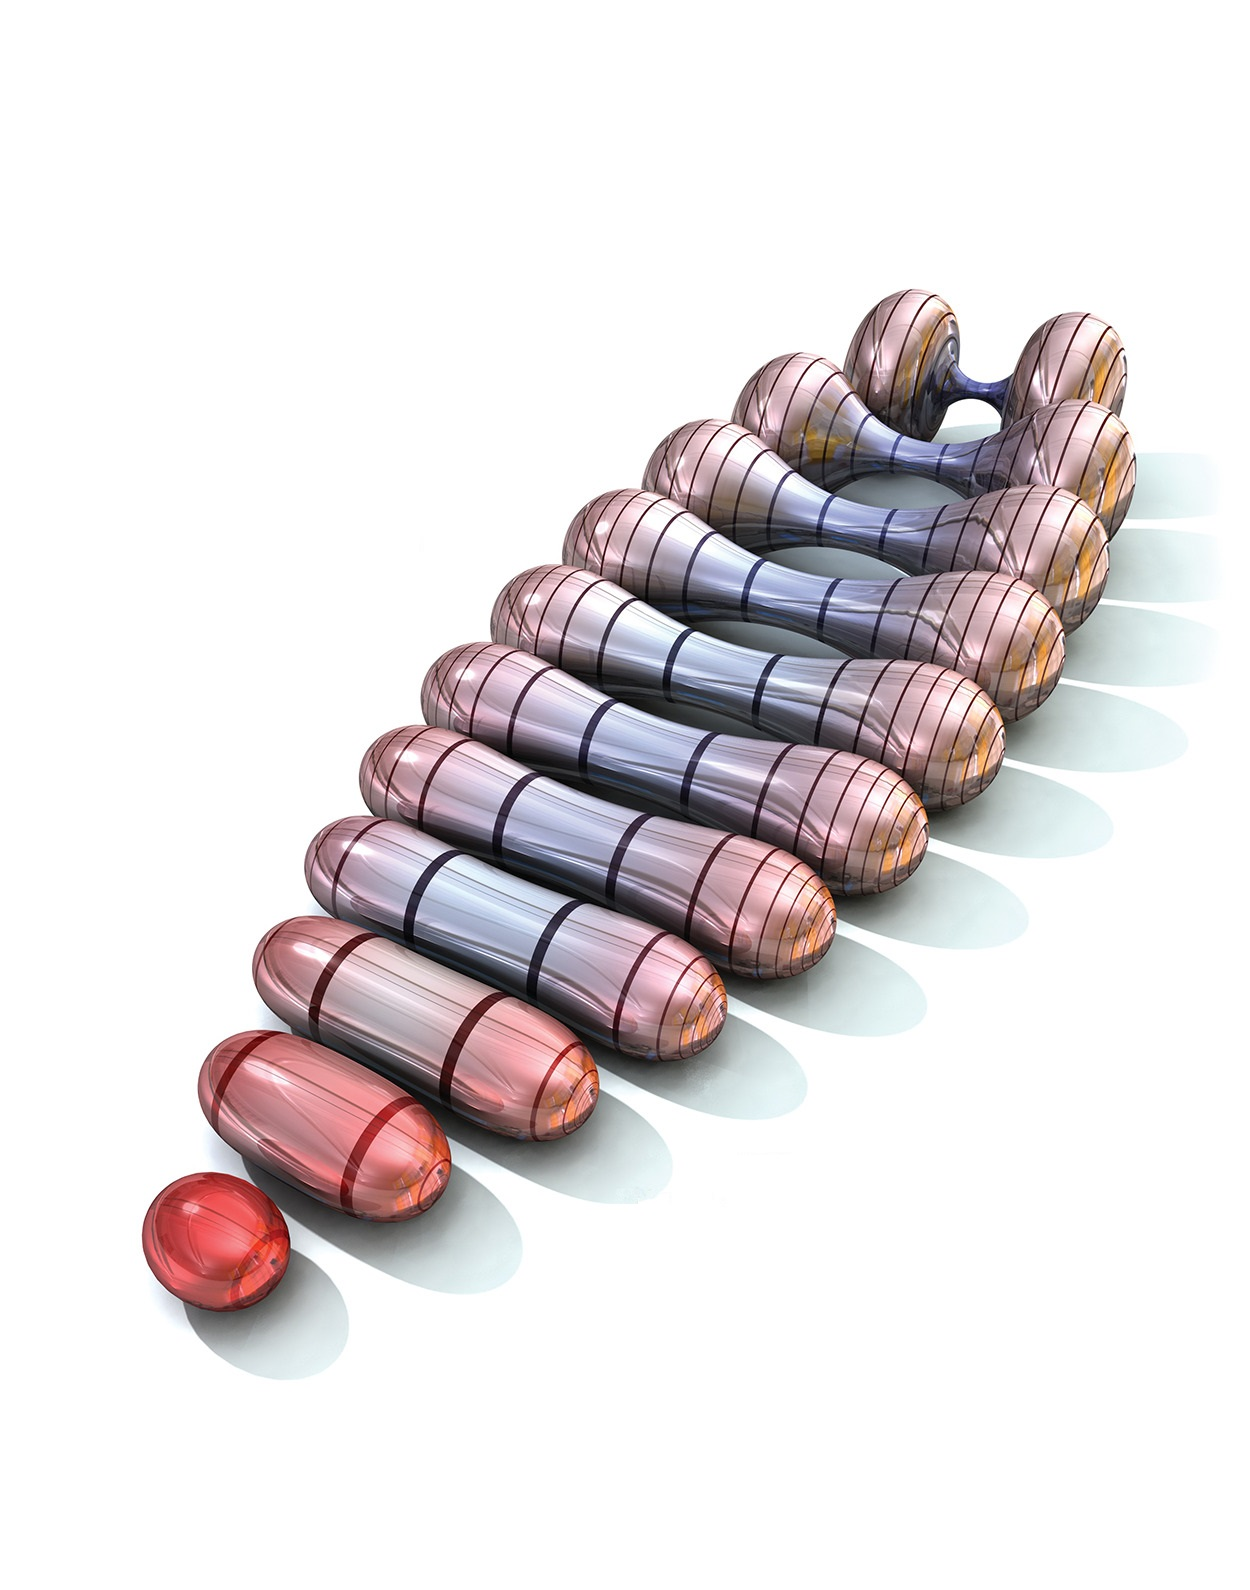
\includegraphics[width=\paperwidth,height=\paperheight,%
keepaspectratio]{background.jpg}%
\vfill
}}}
\fi
\begin{document}
%\AddToShipoutPicture*{\BackgroundPic}
\frontmatter
\pagestyle{empty}
\maketitle

%\let\cleardoublepage\clearpage
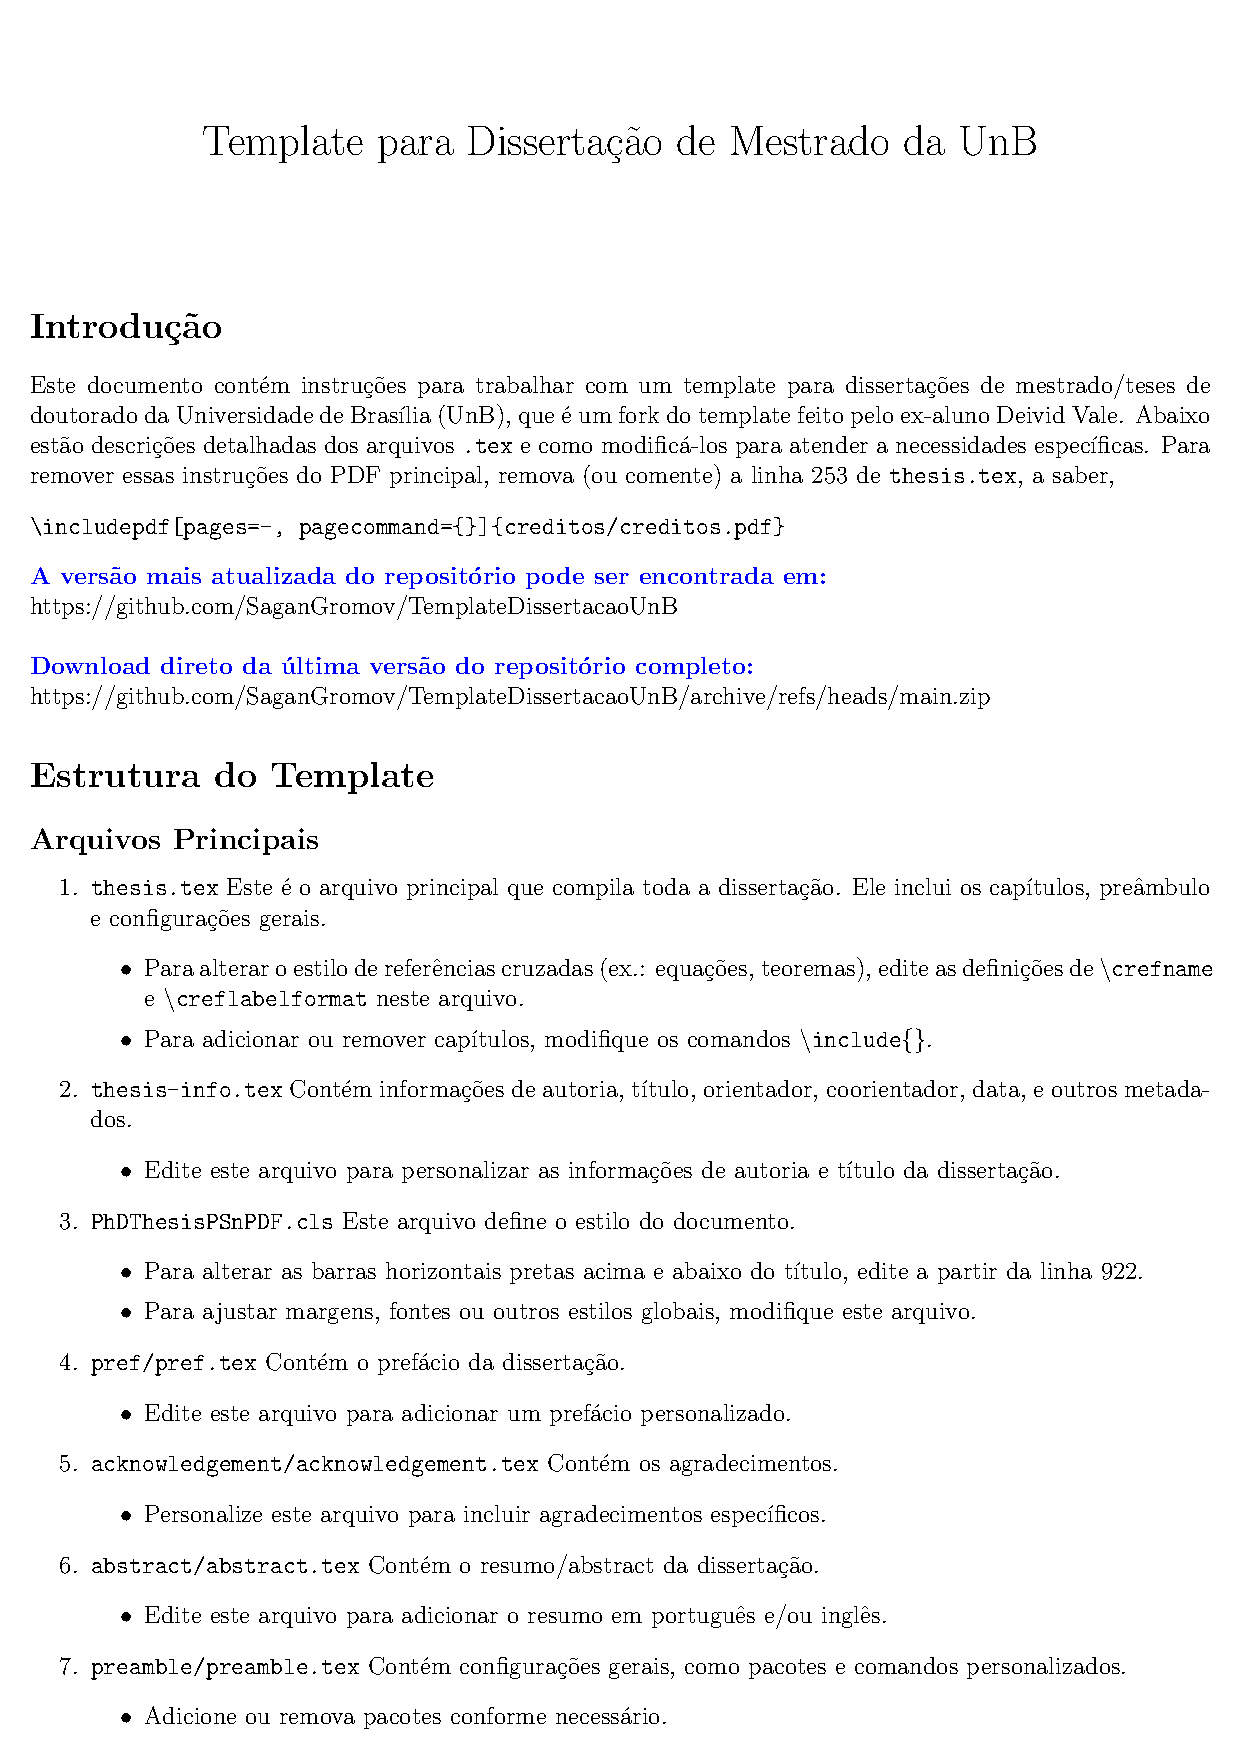
\includepdf[pages=-, pagecommand={}]{creditos/creditos.pdf}
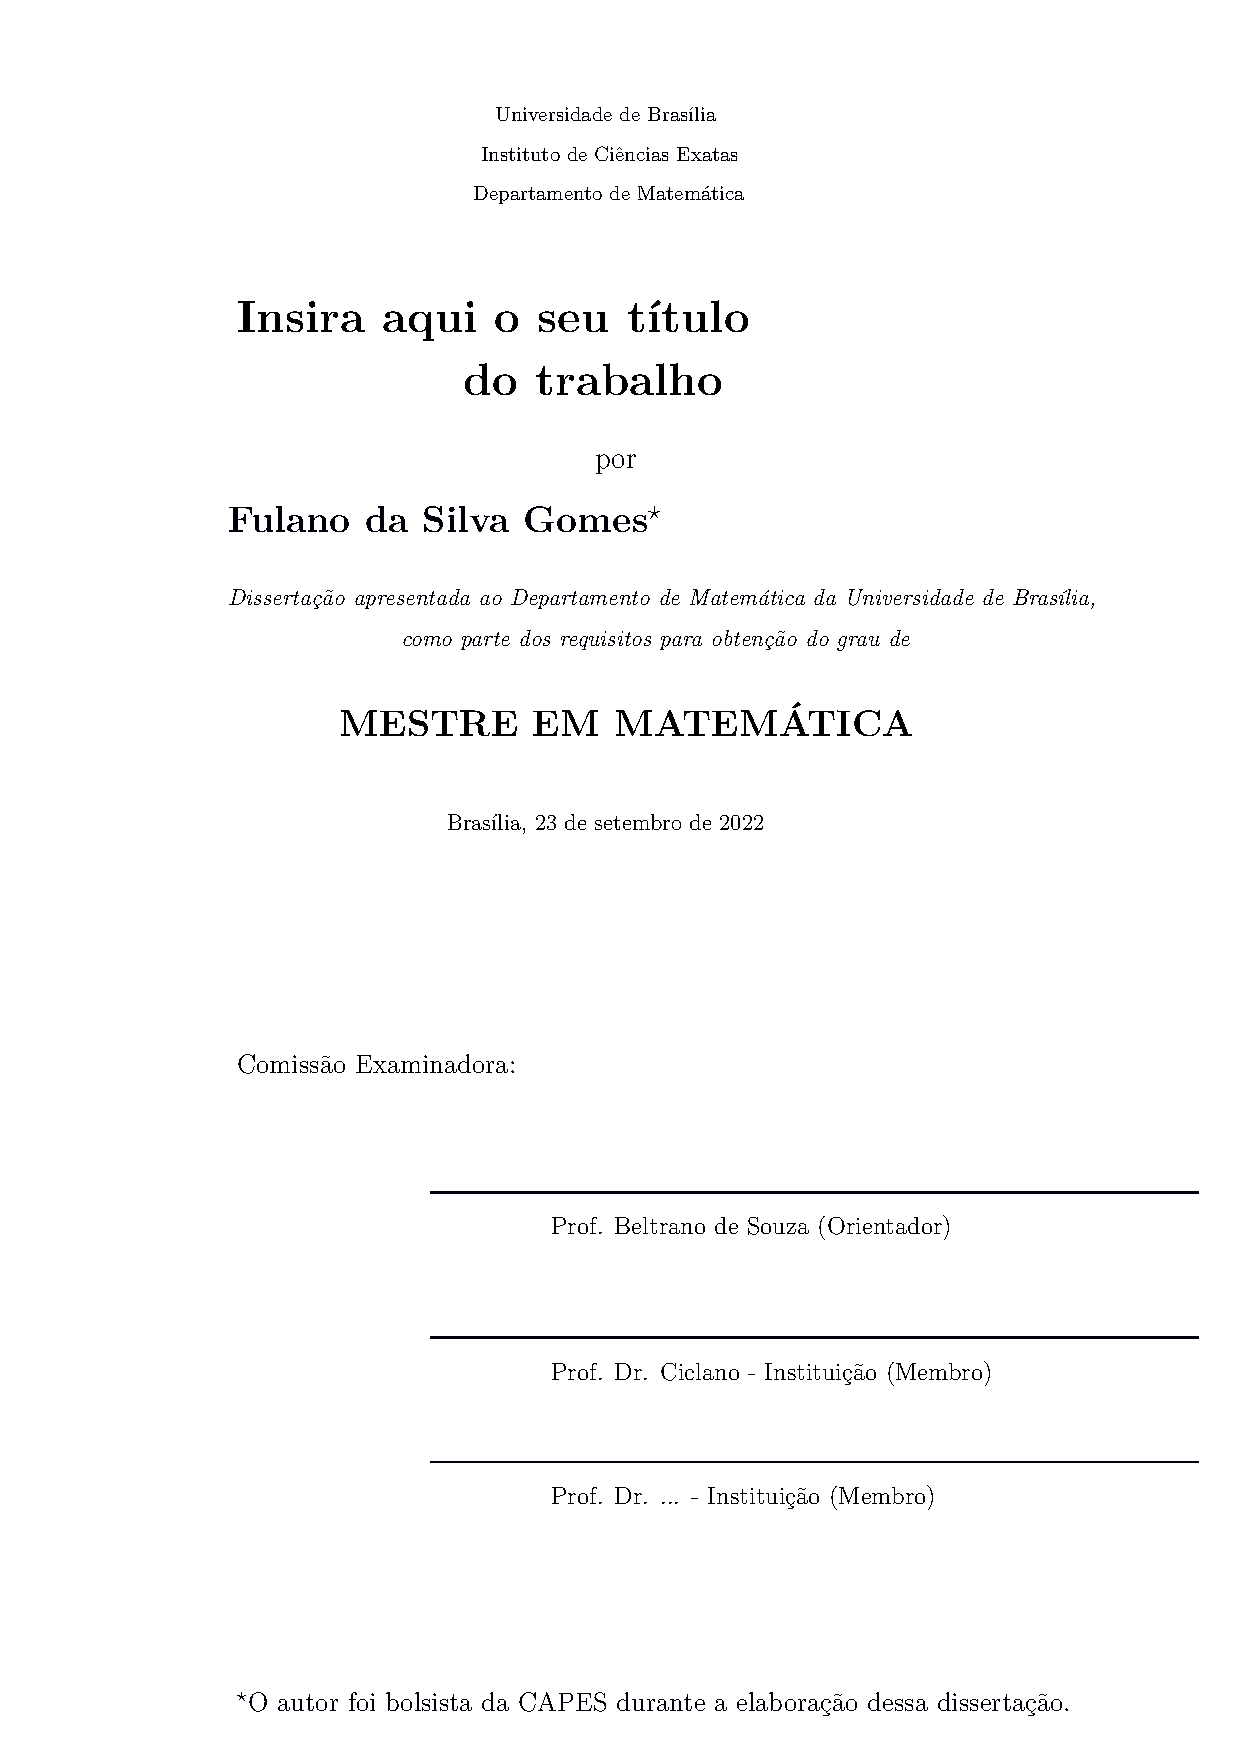
\includepdf[pages=1, pagecommand={}]{assets/codigo_segunda_pagina/sec.pdf}
\thispagestyle{plain}
%\let\cleardoublepage\clearpage
%\includepdf[pages=1, pagecommand={}]{Assets/lbc1}
%\let\cleardoublepa'ge\clearpage
% ******************************* Thesis Dedidcation ********************************
\newgeometry{bottom=0.1in,top=0in,left=0.3in,right=0.3in}
\begin{dedication}

\vspace{7.1cm}
%\PlaceText{69mm}{11mm}{ \color{gal}\noindent\makebox[\linewidth]{\rule{2\paperwidth}{1pt}}}
\PlaceText{69mm}{12.5mm}{ \color{\COR}\noindent\makebox[\linewidth]{\rule{2\paperwidth}{1pt}}}
\PlaceText{13mm}{79}{\huge{\textbf{\textcolor{gal}{Dedico esse trabalho a Carl Edward Sagan.}}}}
\PlaceText{69mm}{33mm}{ \color{\COR}\noindent\makebox[\linewidth]{\rule{2\paperwidth}{1pt}}}


\begin{textblock*}{5cm}(0.5cm,4cm)

\epigraph{\large\textit{What an astonishing thing a book is. It's a flat object made from a tree with flexible parts on which are imprinted lots of funny dark squiggles. But one glance at it and you're inside the mind of another person, maybe somebody dead for thousands of years. Across the millennia, an author is speaking clearly and silently inside your head, directly to you. Writing is perhaps the greatest of human inventions, binding together people who never knew each other, citizens of distant epochs. Books break the shackles of time. A book is proof that humans are capable of working magic.}}{\textbf{Carl Sagan \\}}


\epigraph{\large\textit{We are a way for the Cosmos to know itself.}}{\textbf{Carl Sagan \\}}


\epigraph{\large\textit{If you wish to make an apple pie from scratch, you must first invent the universe.}}{\textbf{Carl Sagan \\}}





\end{textblock*}

\begin{textblock*}{5cm}(12.5cm,4cm)

\epigraph{\large\textit{Extraordinary claims require extraordinary evidence.}}{\textbf{Carl Sagan \\}}


\epigraph{\large\textit{Who is more humble? The scientist who looks at the universe with an open mind and accepts whatever the universe has to teach us, or somebody who says everything in this book must be considered the literal truth and never mind the fallibility of all the human beings involved?}}{\textbf{Carl Sagan \\}}

\epigraph{\large\textit{Imagination will often carry us to worlds that never were. But without it we go nowhere.}}{\textbf{Carl Sagan \\}}

\epigraph{\large\textit{It pays to keep an open mind, but not so open your brains fall out.}}{\textbf{Carl Sagan \\}}

\epigraph{\large\textit{For me, it is far better to grasp the Universe as it really is than to persist in delusion, however satisfying and reassuring.}}{\textbf{Carl Sagan \\}}


\iffalse

\epigraph{\large\textit{One of the saddest lessons of history is this: If we’ve been bamboozled long enough, we tend to reject any evidence of the bamboozle. We’re no longer interested in finding out the truth. The bamboozle has captured us. It’s simply too painful to acknowledge, even to ourselves, that we’ve been taken. Once you give a charlatan power over you, you almost never get it back.}}{\textbf{Carl Sagan \\}}

\fi


\end{textblock*}





\newpage

\newgeometry{bottom=0.1in,top=0in,left=0.5in,right=0.5in}
\vbox{
\begin{textblock*}{5cm}(12.5cm,0cm) % {block width} (coords) 
%
\epigraph{\large\textit{Aut viam inveniam aut faciam.}}{\textbf{Hannibal Barca \\}}

\epigraph{\large\textit{Only those who will risk going too far can possibly find out how far one can go.}}{\textbf{T. S. Elliot \\}}


\epigraph{\large\textit{There is no royal road to geometry.}}{\textbf{Euclid \\}}

\epigraph{\large\textit{We are absurdly accustomed to the miracle of a few written signs being able to contain immortal imagery, involutions of thought, new worlds with live people, speaking, weeping, laughing. We take it for granted so simply that in a sense, by the very act of brutish routine acceptance, we undo the work of the ages, the history of the gradual elaboration of poetical description and construction, from the treeman to Browning, from the caveman to Keats. What if we awake one day, all of us, and find ourselves utterly unable to read? I wish you to gasp not only at what you read but at the miracle of its being readable.
}}{\textbf{Vladimir Nabokov \\}}



\end{textblock*}

\begin{textblock*}{5cm}(0.5cm,0cm) % {block width} (coords) 

\epigraph{\large\textit{Mathematics is not about numbers, equations, computations, or algorithms: it is about understanding.}}{\textbf{William Thurston \\}}

%\epigraph{\large\textit{Aut viam inveniam aut faciam.}}{\textbf{Hannibal Barca \\}}
\iffalse
\epigraph{\textit{Imagination will often carry us to worlds that never were. But without it we go nowhere.}}{\textbf{Carl Sagan \\}}
\fi

\iffalse
\epigraph{\large\textit{If people do not realize that mathematics is simple, it is only because they do not realize how complicated life is.}}{\textbf{John von Neumann\\}}
\fi

\epigraph{\large\textit{Wir müssen wissen. \newline Wir werden wissen. }}{\textbf{David Hilbert\\}}

\epigraph{\large\textit{If I have seen further it is only by standing on the shoulders of giants.}}{\textbf{Isaac Newton\\}}


\FRASE{A human being is part of a whole, called by us the \quotes{Universe}, a part limited in time and space. He experiences himself, his thoughts and feelings, as something separated from the rest - a kind of optical delusion of his consciousness. This delusion is a kind of prison for us, restricting us to our personal desires and to affection for a few persons nearest us. Our task must be to free ourselves from this prison by widening our circles of compassion to embrace all living creatures and the whole of nature in its beauty.}{Albert Einstein}

%\epigraph{\textit{Great men are forged in fire. It is the privillege of lesser men to light the flame.}}{\textbf{Isaac Newton\\}}
\PlaceText{3mm}{799}{\textcolor{gal}{\large\textbf{\textit{Great men are forged in fire. It is the privilege of lesser men to light the flame.}}}}

\PlaceText{85mm}{821}{\textcolor{gal}{\small\textbf{\textit{Steven Moffat}}}}







\iffalse
\epigraph{\textit{The Communists disdain to conceal their views and aims. They openly declare that their ends can be attained only by the forcible overthrow of all existing social conditions. Let the ruling classes tremble at a Communistic revolution. The proletarians have nothing to lose but their chains. They have a world to win. Working Men of All Countries, Unite!}}{\textbf{Karl Marx\\}}
\fi







\end{textblock*}
\vspace{-6cm}



\iffalse
\epigraph{\large\textit{Only those who will risk going too far can possibly find out how far one can go.}}{\textbf{T. S. Elliot \\}}

\epigraph{\large\textit{What an astonishing thing a book is. It's a flat object made from a tree with flexible parts on which are imprinted lots of funny dark squiggles. But one glance at it and you're inside the mind of another person, maybe somebody dead for thousands of years. Across the millennia, an author is speaking clearly and silently inside your head, directly to you. Writing is perhaps the greatest of human inventions, binding together people who never knew each other, citizens of distant epochs. Books break the shackles of time. A book is proof that humans are capable of working magic.}}{\textbf{Carl Sagan \\}}

\epigraph{\large\textit{Extraordinary claims require extraordinary evidence.}}{\textbf{Carl Sagan \\}}
\epigraph{\large\textit{Mathematics is not about numbers, equations, computations, or algorithms: it is about understanding.}}{\textbf{William Thurston \\}}
\fi
}
\end{dedication}
\restoregeometry

%\let\cleardoublepage\clearpage
% ************************** Thesis Acknowledgements **************************



\PlaceText{69mm}{39mm}{ \color{gal}\noindent\makebox[\linewidth]{\rule{2\paperwidth}{1pt}}}

\PlaceText{69mm}{11mm}{ \color{gal}\noindent\makebox[\linewidth]{\rule{2\paperwidth}{1pt}}}

\PlaceText{69mm}{30mm}{\Huge \textcolor{gal}{\textbf{Agradecimentos}} }

\vspace{2.5cm}



\begin{enumerate}[
leftmargin=0pt, itemindent=20pt,
labelwidth=15pt, labelsep=5pt, listparindent=0.7cm,
align=left]


\item[] \lettrine[nindent=2em,lines=1]{P}\ rimeiramente, ...

Agradeço ...!

Agradeço a ...! 





\end{enumerate}




%\let\cleardoublepage\clearpage
% ************************** Thesis Abstract *****************************
% Segundo as regras da Universidade de Brasília, mesmo que a dissertação/tese seja escrita em inglês deve conter um resumo em Português e em Inglês.


\PlaceText{69mm}{39mm}{ \color{gal}\noindent\makebox[\linewidth]{\rule{2\paperwidth}{1pt}}}

\PlaceText{69mm}{11mm}{ \color{gal}\noindent\makebox[\linewidth]{\rule{2\paperwidth}{1pt}}}

\PlaceText{85mm}{28.5mm}{\Huge \textcolor{gal}{\textbf{Resumo}} }

\vspace{2.5cm}


Neste trabalho fazemos um estudo ... \par 
%\vspace{1cm}
\textbf{Palavras-chave:} fluxo de Ricci, sólitons de Ricci, estimativas de curvatura, tensor de Weyl, variedades quadridimensionais.

\iffalse

Neste trabalho apresentamos um estudo de sólitons de Ricci quadridimensionais gradiente completos e shrinking. Apresentamos detalhadamente as demonstrações (de autoria de Huai-Dong Cao, Ernani Ribeiro Jr, e Detang Zhou, expostas originalmente em \mycitep{ernani}) de dois teoremas que garantem certas classificações topológicas e controles na curvatura de Ricci ou curvatura Riemanniana, desde que sejam satisfeitas certas estimativas pontuais sobre as partes duais ou anti-auto-duais do tensor de Einstein ou um certo controle sobre a curvatura escalar.
\fi

\newpage 

\PlaceText{69mm}{39mm}{ \color{gal}\noindent\makebox[\linewidth]{\rule{2\paperwidth}{1pt}}}

\PlaceText{69mm}{11mm}{ \color{gal}\noindent\makebox[\linewidth]{\rule{2\paperwidth}{1pt}}}

\PlaceText{87mm}{29mm}{\Huge \textcolor{gal}{\textbf{Abstract}} }

\vspace{2.5cm}

In this work, we provide a study of complete gradient shrinking Ricci solitons of dimension $4$. We present in detail the proofs (by Huai-Dong Cao, Ernani Ribeiro Jr, and Detang Zhou, originally exposed in \mycitep{ernani}) of two theorems that guarantee geometrical classifications and controls on the Ricci or Riemannian curvature, provided that pointwise estimates on the self-dual or anti-self-dual parts of the Weyl tensor or a certain control on the scalar curvature in terms of the soliton's potential function are satisfied.\par
\textbf{Keywords:} Ricci flow, Ricci solitons, curvature estimates, Weyl tensor, four-manifolds. 


\iffalse
\begin{resumo}
    Resumo em Português.
\end{resumo}


\begin{abstract}
This is where you write your abstract ...
\end{abstract}
\fi





\pagestyle{MyFancy}
% *********************** Adding TOC and List of Figures ***********************

\tableofcontents


%\listoftables

% \printnomenclature[space] space can be set as 2em between symbol and description
%\printnomenclature[3em]

%\printnomenclature

% ******************************** Main Matter *********************************
\mainmatter
%\include{pref/pref}
%!TEX root = ../thesis.tex
%*******************************************************************************
%*********************************** First Chapter *****************************
%*******************************************************************************
\fancypagestyle{plain}{%              
\fancyhf{}
%\renewcommand{\subsectionmark}[1]{%
  %\markright{\MakeUppercase{\thesubsection\ \ \ \ #1 }}}
  %\renewcommand{\chaptermark}[1]{\markboth{teste ##1}{}}
  %\renewcommand{\sectionmark}[1]{\markright{\thesection\ ##1}}

  %\renewcommand{\headrulewidth}{0.7pt}
    %\fancyhead[LO]{\bfseries  \nouppercase{CAPÍTULO \thechapter}  }
      \renewcommand\footrule{%

 \color{\corcaps}\noindent\makebox[\linewidth]{\rule{\paperwidth}{1pt}}
}

      %\renewcommand\headrule{%

 %\color{\corcaps}\noindent\makebox[\linewidth]{\rule{\paperwidth}{1pt}}
%}
        %\fancyhead[LO]{\bfseries}
        \fancyfoot[RO]{\bfseries Página \thepage \ de \pageref*{LastPage}}
    %\fancyhead[RO]{\bfseries \nouppercase \leftmark}
    }
    
\fancypagestyle{MyFancy}{%              
\fancyhf{}
%\renewcommand{\subsectionmark}[1]{%
  %\markright{\MakeUppercase{\thesubsection\ \ \ \ #1 }}}
  %\renewcommand{\chaptermark}[1]{\markboth{##1}{}}
  %\renewcommand{\sectionmark}[1]{\markright{\thesection\ ##1}}
  %\renewcommand{\headrulewidth}{0.7pt}
  \renewcommand{\sectionmark}[1]{ \markright{ ##1}}
  \renewcommand\headrule{%

 \color{\corcaps}\noindent\makebox[\linewidth]{\rule{\paperwidth}{1pt}}
}
  \renewcommand\footrule{%

 \color{\corcaps}\noindent\makebox[\linewidth]{\rule{\paperwidth}{1pt}}
}
	%\fancyhead[RO]{\bfseries \rightmark}
	%\fancyhead[LO]{\bfseries \nouppercase{\thesubsection} }
    \fancyhead[RO]{\bfseries \nouppercase{\rightmark}  
    }
    \fancyfoot[RO]{\bfseries Página \thepage \ de \pageref*{LastPage}}
    \fancyfoot[LO]{\bfseries }
    %\fancyhead[RO]{\bfseries \nouppercase \leftmark}
    }
\addtocounter{page}{9}
\pagestyle{MyFancy}

\color{gal}
\chapter*{Introdução}\addcontentsline{toc}{chapter}{Introdução}\markboth{Introdução}{Introdução}
\label{cap:intReal}



\PlaceText{69mm}{35mm}{ \color{gal}\noindent\makebox[\linewidth]{\rule{2\paperwidth}{1pt}}}

\PlaceText{69mm}{63mm}{ \color{gal}\noindent\makebox[\linewidth]{\rule{2\paperwidth}{1pt}}}

\PlaceText{15mm}{12mm}{ \color{white}\noindent\makebox[\linewidth]{\rule{2\paperwidth}{10pt}}}

\iffalse
\color{red}

\begin{todolist}

\boldmath
    % pra marcar o item como feito é só colocar \item[\done]
    \bf{
    %\item[\done] ainda não feito
        \item[\done] terminar resumo
        \item[\done] palavras-chave
	\item[\done] terminar a introdução
	\item[\done] terminar de arrumar as referências
	\item arrumar pontuação das equações
	}
\end{todolist}




\fi

\color{black}
\lettrine[nindent=2em,lines=1]{E}m geral, ...

%!TEX root = ../thesis.tex
%*******************************************************************************
%*********************************** First Chapter *****************************
%*******************************************************************************
%\addtocounter{page}{7}
\fancypagestyle{plain}{%              '
\fancyhf{}
%\renewcommand{\subsectionmark}[1]{%
  %\markright{\MakeUppercase{\thesubsection\ \ \ \ #1 }}}
  %\renewcommand{\chaptermark}[1]{\markboth{teste ##1}{}}
  %\renewcommand{\sectionmark}[1]{\markright{\thesection\ ##1}}
  %\renewcommand{\headrulewidth}{0.7pt}
    %\fancyhead[LO]{\bfseries  \nouppercase{CAPÍTULO \thechapter}  }
        \fancyfoot[RO]{\bfseries Página \thepage \ de \pageref*{LastPage}}
    %\fancyhead[RO]{\bfseries \nouppercase \leftmark}
    }

\fancypagestyle{MyFancy}{%              
\fancyhf{}
%\renewcommand{\subsectionmark}[1]{%
  %\markright{\MakeUppercase{\thesubsection\ \ \ \ #1 }}}
  %\renewcommand{\chaptermark}[1]{\markboth{##1}{}}
  %\renewcommand{\sectionmark}[1]{\markright{\thesection\ ##1}}
  %\renewcommand{\headrulewidth}{0.7pt}
  \color{gal}
  \renewcommand{\sectionmark}[1]{ \markright{\textcolor{gal}{##1}}}
  \renewcommand\headrule{%

 \color{\corcaps}\noindent\makebox[\linewidth]{\rule{\paperwidth}{1pt}}
}
  \renewcommand\footrule{%

 \color{\corcaps}\noindent\makebox[\linewidth]{\rule{\paperwidth}{1pt}}
}
	%\fancyhead[RO]{\bfseries \rightmark}
	\fancyhead[LO]{\textcolor{gal}{\bfseries \nouppercase{\thesubsection} }}
    \fancyhead[RO]{\textcolor{gal}{\bfseries \nouppercase{\rightmark}}}
    \fancyfoot[RO]{\textcolor{gal}{\bfseries Página \thepage \ de \pageref*{LastPage}}}
    %\fancyfoot[LO]{\bfseries CAPÍTULO \thechapter}
    %\fancyhead[RO]{\bfseries \nouppercase \leftmark}
    }
\pagestyle{MyFancy}
\color{gal}
\chapter{Preliminary Concepts and Notations}
\markboth{Preliminaries}{Concepts}  
\label{cap:preliminares}



\ifpdf
    \graphicspath{{Chapter1/figs/Raster/}{Chapter1/figs/PDF/}{Chapter1/figs/}}
\else
    \graphicspath{{Chapter1/figs/Vector/}{Chapter1/figs/}}
\fi
%********************************** %First Section  **************************************

\PlaceText{69mm}{39mm}{ \color{gal}\noindent\makebox[\linewidth]{\rule{2\paperwidth}{1pt}}}

\PlaceText{69mm}{79mm}{ \color{gal}\noindent\makebox[\linewidth]{\rule{2\paperwidth}{1pt}}}

\color{black}


The purpose of this chapter is to establish the foundational concepts, notations, and conventions that will be used throughout this work. While we aim to make the exposition as self-contained as possible, some familiarity with basic concepts in Riemannian geometry and differentiable manifolds is assumed. Below, we provide a brief overview of the key ideas.

\section{Riemannian Manifolds}
\PlaceText{15mm}{13mm}{ \color{white}\noindent\makebox[\linewidth]{\rule{2\paperwidth}{10pt}}}
\vspace{-1.5cm}
\begin{oobs}
This section introduces the basic definitions and properties of Riemannian manifolds, including the notions of metric tensors, tangent spaces, and smooth maps. We also discuss the importance of coordinate charts and local frames in understanding the geometry of manifolds.
\end{oobs}

\begin{oobs}
We adopt standard notations for Riemannian geometry. For instance, the metric tensor is denoted by \( g \), and the Levi-Civita connection is denoted by \( \nabla \). The curvature tensor, Ricci tensor, and scalar curvature are also introduced with their respective notations.
\end{oobs}

\begin{deff}
A Riemannian manifold is a differentiable manifold \( \mathcal{M} \) equipped with a smooth, positive-definite metric tensor \( g \). This metric allows us to define notions of angles, lengths, and volumes on \( \mathcal{M} \).
\end{deff}

\begin{teorema}[Fundamental Theorem of Riemannian Geometry]
On a Riemannian manifold \( (\mathcal{M}, g) \), there exists a unique torsion-free connection \( \nabla \) that is compatible with the metric \( g \). This connection is called the Levi-Civita connection.
\end{teorema}

\begin{demm}
The proof involves verifying the existence and uniqueness of the Levi-Civita connection using the Koszul formula.
\end{demm}

\section{Tensors}
\vspace{-0.7cm}
This section provides an overview of tensor algebra and calculus, focusing on the types of tensors commonly encountered in Riemannian geometry. Topics include tensor products, contractions, and the metric-induced isomorphisms between tensors of different types.

\begin{deff}
A tensor of type \( (r, s) \) on a vector space \( V \) is a multilinear map \( T: V^* \times \cdots \times V^* \times V \times \cdots \times V \to \mathbb{R} \), where \( V^* \) is the dual space of \( V \).
\end{deff}

\begin{oobs}
Tensors can be represented in a chosen basis, and their components transform according to specific rules under a change of basis. This property makes tensors coordinate-independent objects.
\end{oobs}

\begin{proposicao}
The space of tensors of type \( (r, s) \) on a vector space \( V \) is a finite-dimensional vector space. Its dimension depends on the dimension of \( V \) and the values of \( r \) and \( s \).
\end{proposicao}

\section{Differential Forms}
Differential forms are a special class of tensors that are completely antisymmetric. They play a central role in integration on manifolds and in the formulation of Stokes' theorem.

\begin{deff}
A differential form of degree \( k \) on a manifold \( \mathcal{M} \) is a completely antisymmetric tensor field of type \( (0, k) \).
\end{deff}

\begin{namedthm}{Theorem}[Stokes' Theorem]
Let \( \mathcal{M} \) be an oriented manifold with boundary \( \partial \mathcal{M} \), and let \( \omega \) be a compactly supported \( (n-1) \)-form on \( \mathcal{M} \). Then,
\[
\int_{\mathcal{M}} d\omega = \int_{\partial \mathcal{M}} \omega.
\]
\end{namedthm}

\section{Additional Topics}
This section briefly introduces advanced topics such as the Hodge star operator, Laplacians, and Bochner's formula, which are essential tools in modern Riemannian geometry.

\begin{deff}
The Hodge star operator \( \star \) maps \( k \)-forms to \( (n-k) \)-forms on an \( n \)-dimensional Riemannian manifold. It is defined such that
\[
\alpha \wedge \star \beta = g(\alpha, \beta) \, \mathrm{vol},
\]
where \( \mathrm{vol} \) is the volume form.
\end{deff}

\begin{teorema}[Bochner's Formula]
On a Riemannian manifold, the Laplacian of a function \( f \) satisfies
\[
\Delta f = \text{div}(\nabla f),
\]
where \( \Delta \) is the Laplace-Beltrami operator.
\end{teorema}

\begin{demm}
The proof involves expressing the Laplacian in local coordinates and using the properties of the Levi-Civita connection.
\end{demm}
%!TEX root = ../thesis.tex
%*******************************************************************************
%****************************** Second Chapter *********************************
%************************f*******************************************************
%\addtocounter{page}{7}
\pagestyle{MyFancy}
\color{gal}
\chapter{O fluxo de Ricci}
\label{cap:OFLUXO}

\PlaceText{69mm}{35mm}{ \color{gal}\noindent\makebox[\linewidth]{\rule{2\paperwidth}{1pt}}}

\PlaceText{69mm}{79mm}{ \color{gal}\noindent\makebox[\linewidth]{\rule{2\paperwidth}{1pt}}}

\PlaceText{15mm}{13mm}{ \color{white}\noindent\makebox[\linewidth]{\rule{2\paperwidth}{10pt}}}

\color{black}

O conteúdo deste capítulo foi substituído por texto genérico para preservar a confidencialidade do trabalho original. A seguir, apresentamos uma visão geral genérica sobre o fluxo de Ricci.

\section{Motivação e exemplos}

O fluxo de Ricci é uma ferramenta matemática poderosa usada para estudar a geometria e a topologia das variedades. Ele foi introduzido por Richard Hamilton na década de 1980 e desempenhou um papel crucial na prova da Conjectura de Poincaré por Grigori Perelman.

\subsection{Definição do fluxo de Ricci}

O fluxo de Ricci é descrito pela seguinte equação diferencial parcial:
\[
\frac{\partial g_{ij}}{\partial t} = -2 \, \mathrm{Ric}_{ij},
\]
onde \( g_{ij} \) é a métrica Riemanniana e \( \mathrm{Ric}_{ij} \) é o tensor de Ricci associado.

\subsection{Propriedades gerais}

O fluxo de Ricci pode ser interpretado como uma deformação da métrica Riemanniana ao longo do tempo, suavizando irregularidades na curvatura da variedade. Ele é frequentemente comparado à equação do calor, que distribui uniformemente a temperatura em um objeto.

\section{Sólitons de Ricci}

Os sólitons de Ricci são soluções especiais do fluxo de Ricci que evoluem apenas por difeomorfismos e mudanças de escala. Eles desempenham um papel importante no estudo de singularidades do fluxo.

\subsection{Definição de sólitons}

Um sóliton de Ricci é uma solução da forma:
\[
\mathrm{Ric} + \nabla^2 f = \lambda g,
\]
onde \( f \) é uma função suave, \( \lambda \) é uma constante, e \( g \) é a métrica Riemanniana.

\subsection{Classificação de sólitons}

Os sólitons de Ricci podem ser classificados em três tipos:
\begin{itemize}
    \item \textbf{Shrinking}: \( \lambda > 0 \)
    \item \textbf{Steady}: \( \lambda = 0 \)
    \item \textbf{Expanding}: \( \lambda < 0 \)
\end{itemize}

\section{Singularidades no fluxo de Ricci}

As singularidades são um aspecto fundamental do estudo do fluxo de Ricci. Elas ocorrem quando a curvatura da métrica se torna infinita em tempo finito.

\subsection{Tipos de singularidades}

As singularidades podem ser classificadas em diferentes tipos, dependendo do comportamento da curvatura:
\begin{itemize}
    \item \textbf{Tipo I}: A curvatura cresce de forma controlada.
    \item \textbf{Tipo II}: A curvatura cresce de forma mais rápida e descontrolada.
\end{itemize}

\subsection{Resolução de singularidades}

Para lidar com as singularidades, técnicas como o "blow-up" são usadas para analisar o comportamento local da métrica perto do ponto de singularidade.

\section{Aplicações do fluxo de Ricci}

O fluxo de Ricci tem aplicações em várias áreas da matemática e da física. Ele é usado para estudar a geometria das variedades, resolver problemas em topologia e até mesmo em teorias físicas como a relatividade geral.

\subsection{Conjectura de Poincaré}

A aplicação mais famosa do fluxo de Ricci foi na prova da Conjectura de Poincaré, um dos problemas do Milênio, resolvido por Grigori Perelman.

\subsection{Geometrização de Thurston}

O fluxo de Ricci também foi usado para abordar a Conjectura de Geometrização de Thurston, que generaliza a Conjectura de Poincaré para dimensões superiores.

\section{Conclusão}

O fluxo de Ricci é uma ferramenta poderosa que conecta a geometria, a análise e a topologia. Ele continua sendo uma área ativa de pesquisa, com muitas questões abertas e aplicações potenciais.

%\include{Chapter4/chapter4}
%\include{Chapter5/chapter5}
%\include{Chapter6/chapter6}
%\include{Chapter7/chapter7}



% ********************************** Back Matter *******************************
% Backmatter should be commented out, if you are using appendices after References
%\backmatter

% ********************************** Bibliography ******************************
\fancypagestyle{plain}{%              
\fancyhf{}
%\renewcommand{\subsectionmark}[1]{%
  %\markright{\MakeUppercase{\thesubsection\ \ \ \ #1 }}}
  %\renewcommand{\chaptermark}[1]{\markboth{teste ##1}{}}
  %\renewcommand{\sectionmark}[1]{\markright{\thesection\ ##1}}
  %\renewcommand{\headrulewidth}{0.7pt}
    %\fancyhead[LO]{\bfseries  \nouppercase{CAPÍTULO \thechapter}  }
      \renewcommand\footrule{%

 \color{\corcaps}\noindent\makebox[\linewidth]{\rule{\paperwidth}{1pt}}
}
      \renewcommand\headrule{%

 \color{\corcaps}\noindent\makebox[\linewidth]{\rule{\paperwidth}{1pt}}
}
        \fancyhead[LO]{\bfseries BIBLIOGRAFIA}
        \fancyfoot[RO]{\bfseries Página \thepage \ de \pageref*{LastPage}}
    %\fancyhead[RO]{\bfseries \nouppercase \leftmark}
    }

\pagestyle{plain}
\fancypagestyle{plainbib}{%              
\fancyhf{}
%\renewcommand{\subsectionmark}[1]{%
  %\markright{\MakeUppercase{\thesubsection\ \ \ \ #1 }}}
  %\renewcommand{\chaptermark}[1]{\markboth{teste ##1}{}}
  %\renewcommand{\sectionmark}[1]{\markright{\thesection\ ##1}}
  %\renewcommand{\headrulewidth}{0.7pt}
    %\fancyhead[LO]{\bfseries  \nouppercase{CAPÍTULO \thechapter}  }
      \renewcommand\footrule{%

 \color{\corcaps}\noindent\makebox[\linewidth]{\rule{\paperwidth}{1pt}}
}
      \renewcommand\headrule{%

 \color{\corcaps}\noindent\makebox[\linewidth]{\rule{\paperwidth}{1pt}}
}
        \fancyhead[LO]{\bfseries BIBLIOGRAFIA}
        \fancyfoot[RO]{\bfseries Página \thepage \ de \pageref*{LastPage}}
    %\fancyhead[RO]{\bfseries \nouppercase \leftmark}
    }

\pagestyle{plainbib}

\begin{spacing}{0.9}
\color{gal}

\begin{thebibliography}{99}

{\bfseries
\color{teal}
\bibitem{ernani}

\bl{
\textbf{Cao, Huai-Dong; Ribeiro, Ernani, Jr.; Zhou, Detang.} Four-dimensional complete gradient shrinking Ricci solitons. \emph{J. Reine Angew. Math.} 778 (2021), 127--144.
}


\PlaceText{69mm}{35mm}{ \color{gal}\noindent\makebox[\linewidth]{\rule{2\paperwidth}{1pt}}}

\PlaceText{69mm}{57mm}{ \color{gal}\noindent\makebox[\linewidth]{\rule{2\paperwidth}{1pt}}}

\PlaceText{15mm}{16mm}{ \color{white}\noindent\makebox[\linewidth]{\rule{2\paperwidth}{30pt}}}

\vspace{-1.5cm}

\bibitem{ivo}
\bl{
\textbf{Couto, I. T.} About curvature like tensors. Texto encontrado em página pessoal. Disponível em: \href{https://www.asc.ohio-state.edu/terekcouto.1/texts/curvaturelike.pdf}{\textbf{https://www.asc.ohio-state.edu/terekcouto.1/texts/curvaturelike.pdf}}. Acessado em 10 de fevereiro de 2023.
}

\bibitem{ivoIndex}
\bl{
\textbf{Couto, I. T.} Some index computations with curvature tensors. Texto encontrado em página pessoal. Disponível em: \href{https://www.asc.ohio-state.edu/terekcouto.1/texts/index_curvature.pdf}{\textbf{https://www.asc.ohio-state.edu/terekcouto.1/texts/index\_curvature.pdf}}. Acessado em 10 de fevereiro de 2023.
}


\bibitem{jeff}
\bl{
\textbf{Viaclovsky, J. A.} Math 865, Topics in Riemannian Geometry. Notas de aula. Disponível em: \href{https://www.math.uci.edu/~jviaclov/courses/865_Fall_2007.pdf}{\textbf{\url{https://www.math.uci.edu/~jviaclov/courses/865\_Fall\_2007.pdf}}}. Acessado em 10 de fevereiro de 2023. 
}



\bibitem{ivoten}
\bl{
\textbf{Couto, I. T.} A mini-course on tensors. Texto encontrado em página pessoal. Disponível em: \href{https://www.asc.ohio-state.edu/terekcouto.1/texts/tensors.pdf}{\textbf{https://www.asc.ohio-state.edu/terekcouto.1/texts/tensors.pdf}}. Acessado em 10 de fevereiro de 2023.
}


\bibitem{rodney}
\bl{
\textbf{Biezuner, R. J.} Notas de aula de geometria Riemanniana. Texto encontrado em página pessoal. Disponível em: \href{http://150.164.25.15/~rodney/notas_de_aula/geometria_riemanniana.pdf}{\textbf{\url{http://150.164.25.15/~rodney/notas_de_aula/geometria_riemanniana.pdf}}}. Acessado em 10 de fevereiro de 2023.
}




\bibitem{topping}
\bl{
\textbf{Topping, Peter.} Lectures on the Ricci flow. London Mathematical Society Lecture Note Series, 325. \emph{Cambridge University Press, Cambridge,} 2006. x+113 pp. ISBN: 978-0-521-68947-2; 0-521-68947-3.
}

\bibitem{eqpoint}
\bl{
\textbf{Emineti, Manolo; La Nave, Gabriele; Mantegazza, Carlo.} Ricci solitons: the equation point of view. \emph{Manuscrita Math.} \textbf{127} (2008), no. 3, 345--367.
}



\bibitem{petlivro}
\bl{
\textbf{Petersen, Peter.} Riemannian geometry. Second edition. Graduate Texts in Mathematics, 171. Springer, New York, 2006. xvi+401 pp. ISBN: 978-0387-29246-5; 0-387-29246-2.
}



\bibitem{pet1}
\bl{
\textbf{Petersen, Peter; Wylie, William.} On the classification of gradient Ricci solitons. Geom. Topol. \textbf{14} (2010), no. 4, 2277--2300.
}



\bibitem{pet2}
\bl{
\textbf{Petersen, Peter; Wylie, William.} Rigidity of gradient Ricci solitons. Pacific J. Math. \textbf{241} (2009), no. 2, 329--345.
}



\bibitem{chen}
\bl{
\textbf{Chen, Bing-Long.} Strong uniqueness of the Ricci flow. \emph{J. Differential Geom.} \textbf{82} (2009), no. 2, 363--382.
}



\bibitem{caodetang}
\bl{\textbf{Cao, Huai-Dong; Zhou, Detang.} On complete gradient shrinking Ricci solitons. \emph{J. Differential Geom.} \textbf{85} (2010), no. 2, 175--185.
}



\bibitem{derd}
\bl{\textbf{Derdziński, Andrzej.} Self-dual Kähler manifolds and Einstein manifolds of dimension four. \emph{Compositio Math.} \textbf{49} (1983), no. 3, 405--433.}



\bibitem{caotran}
\bl{\textbf{Cao, Xiaodong; Tran, Hung.} The Weyl tensor of gradient Ricci solitons. \textit{Geom. Topol.} \textbf{20} (2016), no. 1, 389--436.
}



\bibitem{peng}
\bl{\textbf{Wu, Peng.} A Weitzenböck formula for canonical metrics on four-manifolds. \emph{Trans. Amer. Math. Soc.} \textbf{369} (2017), no. 2, 1079--1096.}




\bibitem{cutoffartigo}
\bl{
\textbf{Azagra, D.; Ferrera, J.; López-Mesas, F.; Rangel, Y. } Smooth approximation of Lipschitz functions on Riemannian manifolds. \emph{J. Math. Anal. Appl.} \textbf{326} (2007), no. 2, 1370--1378.
}


 
\bibitem{peng33}
\bl{
\textbf{Wu, Jia-Yong; Wu, Peng; Wylie, William.} Gradient shrinking Ricci solitons of half harmonic Weyl curvature. \emph{Calc. Var. Partial Differential Equations} \textbf{57} (2018), no. 5, Paper No. 141, 15 pp.
}




\bibitem{munt}
\bl{
\textbf{Munteanu, Ovidiu; Sesum, Natasa.} On gradient Ricci solitons. \emph{J. Geom. Anal.} \textbf{23} (2013), no. 2, 539--561.
}



\bibitem{munt25}
\bl{
\textbf{Munteanu, Ovidiu; Wang, Jiaping.} Geometry of shrinking Ricci solitons. \emph{Compos. Math.} \textbf{151} (2015), no. 12, 2273--2300.
}



\bibitem{rteo1.2}
\bl{\textbf{Chen, Xiuxiong; Wang, Yuanqi.} On four-dimensional anti-self-dual gradient Ricci solitons. \emph{J. Geom. Anal.} \textbf{25} (2015), no. 2, 1335--1343.}

\bibitem{LeeTop}
\bl{
\textbf{Lee, John M.} Introduction to topological manifolds. Second edition. Graduate Texts in Mathematics, 202. Springer, New York, 2011. xviii+433 pp. ISBN: 978-1-4419-7939-1
}

\bibitem{leesmooth}
\bl{
\textbf{Lee, John M.} Introduction to smooth manifolds. Second edition. Graduate Texts in Mathematics, 218. Springer, New York, 2013. xvi+708 pp. ISBN: 978-1-4419-9981-8 
}

\bibitem{leeriem}
\bl{
\textbf{Lee, John M.} Introduction to Riemannian manifolds. Second edition of [MR1468735]. Graduate Texts in Mathematics, 176. Springer, Cham, 2018. xiii+437 pp. ISBN: 978-3-319-91754-2; 978-3-319-91755-9
}

\bibitem{foster}
\bl{
\textbf{Foster, James; Nightingale, J. David.} A short course in general relativity. Third edition. Springer, New York, 2006. x+292 pp. ISBN: 978-0387-26078-5; 0-387-26078-1.
}

\bibitem{TuRiem}
\bl{
\textbf{Tu, Loring W.} Differential geometry. Connections, curvature, and characteristic classes. Graduate Texts in Mathematics, 275. \emph{Springer, Cham,} 2017. xvi+346 pp. ISBN: 978-3-319-55082-4; 978-3-319-55084-8.
}




\bibitem{kirby}
\bl{\textbf{Kirby, Robion C.} The topology of $4$-manifolds. Lecture Notes in Mathematics, 1374. \emph{Springer-Verlag, Berlin,} 1989. {\rm vi}+108 pp. ISBN: 3-540-51148-2. \iffalse \href{https://mathscinet.ams.org/mathscinet-getitem?mr=1001966}{\textbf{MR1001966}} \fi
}

\bibitem{2ham}
\bl{\textbf{Hamilton, Richard S.} The Ricci flow on surfaces. \emph{Mathematics and general relativity (Santa Cruz, CA, 1986)}, 237--262, Contemp. Math., 71, \emph{Amer. Math. Soc., Providence, RI, } 1988. \iffalse \href{https://mathscinet.ams.org/mathscinet-getitem?mr=954419}{\textbf{MR0954419}} \fi}

\bibitem{3ham}
\bl{
\textbf{Hamilton, Richard S.} Three-manifolds with positive Ricci curvature. \emph{J. Differential Geometry} \textbf{17} (1982), no. 2, 255--306.
}



\bibitem{4ham}
\bl{
\textbf{Hamilton, Richard S.} Four-manifolds with positive curvature operator. \emph{J. Differential Geom.} \textbf{24} (1986), no. 2, 153--179.
}

\bibitem{PerelmanGradiente}
\bl{
\textbf{Perelman, G. Y.} The entropy formula for the Ricci flow and its geometric applications. Preprint, arXiv math/0211159, 2002.
}

\bibitem{HamRicciFlow}
\bl{
\textbf{Chow, Bennett; Lu, Peng; Ni, Lei.} Hamilton's Ricci flow. Graduate Studies in Mathematics, 77. \emph{American Mathematical Society, Providence, RI; Science Press Beijing, New York}, 2006. xxxvi+608 pp. ISBN: 978-0-8218-4231-7; 0-8218-4231-5.
}

\bibitem{MeuWarped}
\bl{
\textbf{Horácio, M.A.R.M.} Produtos warped. Texto encontrado em página pessoal. Disponível em \href{https://github.com/SaganGromov/ProdutosWarped/blob/main/ProdutosWarped.pdf}{\textbf{https://github.com/SaganGromov/ProdutosWarped/blob/main/ProdutosWarped.pdf}}. Acessado em 13 de fevereiro de 2023.
}



\bibitem{McMillan}
\bl{\textbf{McMillan, D. R., Jr.} Some contractible open $3$-manifolds. \emph{Trans. Amer. Math. Soc.} 102 (1962), 373--382. \iffalse \href{https://mathscinet.ams.org/mathscinet-getitem?mr=137105}{\textbf{MR0137105}} \fi}

\iffalse
\bibitem{dodecaedro}
\bl{C.Weber e H.Seifert, \quotes{Die beiden Dodekaedraume,} \emph{Mathematische Zeitschrift} 37, no. 2 (1933)}
\fi

\bibitem{dodecaedro}
\bl{
\textbf{Seifert H., Weber C. } Die beiden Dodekaedraüme, Mathematische Zeitschrift 1933. V. 37. P. 237–253.
}

\bibitem{ArtDodecaedro}
\bl{\textbf{Luminet, J.P., J.R. Weeks, A. Riazuelo, R. Lehoucq, R., and J.P. Uzan.} Dodecahedral space topology as an explanation for weak wide-angle temperaure correlations in the cosmic microwave background. \emph{Nature}, (2003), \textbf{425}, 593-95.}

\bibitem{JohnMorgan}
\bl{
\textbf{Morgan, John W.} Recent progress on the Poincaré conjecture and the classification of 3-manifolds. \emph{Bull. Amer. Math. Soc. (N.S.)} \textbf{42} (2005), no. 1, 57--78.
}


\bibitem{overflow}
\bl{
\textbf{MathOverflow}. Classification of surfaces and the TOP, DIFF and PL categories for manifolds. Disponível em: \href{https://mathoverflow.net/questions/96670/classification-of-surfaces-and-the-top-diff-and-pl-categories-for-manifolds}{\textbf{https://mathoverflow.net/questions/96670/classification-of-surfaces-and-the-top-diff-and-pl-categories-for-manifolds}}. Acessado em 10 de fevereiro de 2023.
}
\iffalse
\bibitem{overflow}
\bl{MathOverflow;} \href{https://mathoverflow.net/questions/96670/classification-of-surfaces-and-the-top-diff-and-pl-categories-for-manifolds}{\textbf{Classification of surfaces and the TOP, DIFF and PL categories for manifolds}}
\fi

\bibitem{NaoCompacto}
\bl{
\textbf{Richards, Ian.} On the classifcation of noncompact surfaces. \emph{Trans. Amer. Math. Soc.} 106 (1963), 259--269.
}

\bibitem{Adam}
\bl{\textbf{Rudnik, Adam Petzet.} \emph{Analysis of the Ricci Flow on Compact Manifolds.} Dissertação de mestrado, Universidade de São Paulo, 2019.}

\bibitem{ChowKnopf}
\bl{\textbf{Chow, Bennett; Knopf, Dan.} The Ricci flow: an introduction. Mathematical Surveys and Monographs, 110. \emph{American Mathematical Society, Providence, RI}, 2004. xii+325 pp. ISBN: 0-8218-3515-7.
}

\iffalse
\bibitem{Lavoyer}
\bl{Lucas Lavoyer, Dissertação de Mestrado} \href{https://mat.unb.br/upload/repositorio/2020_06_24/Dissertacao_Lucas.pdf}{\textbf{On the Maximum Principle and the Ricci flow}}
\fi


\bibitem{DifConf1}
\bl{\textbf{Gomes, J.N.} \emph{Rigidez de superfícies de contato e caracterização de variedades Riemannianas munidas de um campo conforme ou de alguma métrica especial.} Tese de doutorado, Universidade Federal do Ceará, (2012).}

\bibitem{DifConf2}
\bl{\textbf{Sharma, Ramesh.} Almost Ricci solitons and $K$-contact geometry. Monatsh. Math. \textbf{175} (2014), no. 4, 621--628.
}



\bibitem{shin}
\bl{
\textbf{Shin, Jinwoo.} On the classification of 4-dimensional $(m,\rho)$-quasi-Einstein manifolds with harmonic Weyl curvature. \emph{Ann. Global Anal. Geom.} \textbf{51} (2017), no. 4, 379--399.
}

\iffalse
\bibitem{pigola} \bl{Pigola, S.; Rigoli, M.; Rimoldi, M.; Setti, A. G. \textit{Ricci almost solitons}. Ann. Sc. Norm. Super. Pisa Cl. Sci. v. 10 n. 4, 757-799, 2011.}


\bibitem{Ryan} \bl{Ryan, P. J.: Homogeneity and some curvature conditions for hypersurfaces. {\textit {Tohoku Mathematical Journal.}} {\textbf{ 21(3)}}. 363-388, 1969.}

\fi



\bibitem{Revista}
\bl{
\textbf{Mackenzie, Dana.} The Poincaré Conjecture--Proved. \emph{Science, } 314(5807):1848-1849, 2006. Disponível em: \href{https://doi.org/10.1126/science.314.5807.1848}{\bf{DOI: 10.1126/science.314.5807.1848}}.
Acessado em 10 de fevereiro de 2023.}

\bibitem{Permissao}
\bl{
\textbf{Reprints and Permissions, Science, AAAS.} Disponível em: \href{https://www.science.org/content/page/reprints-and-permissions}{\textbf{\url{https://www.science.org/content/page/reprints-and-permissions}}}. Acessado em 10 de fevereiro de 2023. 
}


\bibitem{Ivey}
\bl{
\textbf{Ivey, Thomas.} New examples of complete Ricci solitons. \emph{Proc. Amer. Math. Soc.} \textbf{122} (1994), no. 1, 241--245.
}

\bibitem{PerelmanS}
\bl{
\textbf{Perelman, G. Y.} Ricci flow with surgery on three manifolds. Preprint, ArXiv:math.DG/0303109, 2003.
}

\iffalse
\bibitem{PerelmanS}
\bl{
Grisha Perelman, \emph{Ricci flow with surgery on three manifolds,} ArXiv:math.DG/0303109 (2003).
}
\fi

\bibitem{Naber}
\bl{
\textbf{Naber, Aaron.} Noncompact shrinking four solitons with nonnegative curvature. \emph{J. Reine Angew. Math.} 645 (2010), 125--153.
}

\bibitem{NiWallach}
\bl{
\textbf{Ni, Lei; Wallach, Nolan.} On a classification of gradient shrinking solitons. \emph{Math. Res. Lett.} \textbf{15} (2008), no. 5, 941--955.
}


\bibitem{CaoChenZhu}
\bl{
\textbf{Cao, Huai-Dong; Chen, Bing-Long; Zhu, Xi-Ping.} Recent developments on Hamilton's Ricci flow. \emph{Surveys in differential geometry. Vol. XII. Geometric flows,} 47--112, Surv. Differ. Geom., 12, \emph{Int. Press, Somerville, MA,} 2008.
}

\bibitem{Arnold}
\bl{\textbf{Arnold, Vladimir I.} On Teaching Mathematics. (Polonês) Traduzido do russo por Danuta Śledziewska-Blocka. \emph{Wiadom. Mat.} 37 (2001), 17--26.}


\bibitem{PEN1}
\bl{
\textbf{Penrose, Roger.} The emperor's new mind. Concerning computers, minds, and the laws of physics. Com um prefácio por Martin Gardner. \emph{The Clarendon Press, Oxford University Press, New York,} 1989. {\rm xiv}+466 pp. ISBN: 0-19-851973-7.
}

\bibitem{PEN2}
\bl{
\textbf{Penrose, Roger.} The road to reality. A complete guide to the laws of the universe. \emph{Alfred A. Knopf, Inc., New York,} 2005. xxviii+1099 pp. ISBN: 0-679-45443-8.
}

\bibitem{RIEMANN}
\bl{\textbf{Riemann, Bernhard.} On the Hypothesis Which Lie At the Bases of Geometry. \emph{Nature}. \textbf{8,} 36-37 (1873). \iffalse \href{https://doi.org/10.1038/008036a0}{https://doi.org/10.1038/008036a0} \fi
}

\bibitem{POINCHYP}
\bl{\textbf{Poincaré, Henry.} \quotes{Science and Hypothesis}, \emph{The Value of Science: Essential Writings of Henri Poincaré, } ed. Stephen Jay Gould (New York: The Modern Library 2001), p.56.}

\bibitem{Lob}
\bl{
\textbf{Lobachevsky, Nikolai I.} \emph{The Foundations of Geometry: Works on Non-Euclidean Geometry.} Traduzido do russo por Svetla Petkova. Editado (com uma Introdução) por V. Petkov. Minkowski Institute Press, Montreal.
}

\bibitem{LobD}
\bl{
\textbf{Kragh, Helge.} Geometry and Astronomy: Pre-Einstein Speculations of Non-Euclidean Space. Preprint, ArXiv:physics/12054909, 2012.
}

\bibitem{Kuhnel}
\bl{
\textbf{Kühnel, Wolfgang.} Conformal transformations between Einstein spaces. \emph{Conformal geometry (Bonn, 1985/1986),} 105--146, Aspects Math., E12, \emph{Friedr. Vieweg, Braunschweig,} 1988.
}

\bibitem{Flanders}
\bl{
\textbf{Flanders, Harley.} Differential forms with applications to the physical sciences. Second edition. Dover Books on Advanced Mathematics. \emph{Dover Publications, Inc., New York,} 1989. {\rm xvi}+205 pp. ISBN: 0-486-66169-5.
}



}




\end{thebibliography}

%\bibliographystyle{apalike}
%\bibliographystyle{unsrt} % Use for unsorted references
%\bibliography{References/citacoes}

\end{spacing}

% ********************************** Apêndices ********************************


% *************************************** Index ********************************
\printthesisindex % If index is present

\end{document}
